\documentclass[10pt,letterpaper]{article}

\usepackage[T1]{fontenc}
\usepackage[utf8]{inputenc}
\usepackage{times}
\usepackage{graphicx}
\usepackage{amsmath}
\usepackage{amssymb}
\usepackage{booktabs}
\usepackage{multirow}
\usepackage{array}
\usepackage{url}
\usepackage{microtype}
\usepackage[margin=1in]{geometry}
\usepackage[colorlinks=true,allcolors=blue]{hyperref}
\usepackage{soul}
\usepackage{xcolor}
% soul's \hl (background highlight) fails to compile on complex content
% (math mode, \ref, curly quotes) throughout this revision's new text, so we
% redefine \hl to mark new/changed content with colored text instead, which
% is robust with any content. This is purely a revision-marking aid for the
% reviewer response and is not intended for the camera-ready version.
\renewcommand{\hl}[1]{\textcolor{purple}{#1}}

\newcommand{\code}[1]{\texttt{#1}}

\title{Zero-shot vision-language models underperform supervised baselines in agricultural image classification across 26 datasets and 121 classes}

\author{Earl Ranario, J. Mason Earles\\[4pt]
University of California, Davis\\
\texttt{\{ewranario, jmearles\}@ucdavis.edu}}

\date{}

\begin{document}
\maketitle

\begin{abstract}
Vision-language models (VLMs) are increasingly proposed as general-purpose solutions for visual recognition tasks, yet their reliability for agricultural decision support remains poorly understood. We benchmark a diverse set of open-source and closed-source VLMs on 26 agricultural image classification datasets from the AgML (\url{https://project-agml.github.io/}) collection, spanning 121 classes and 248,000 images across plant disease, pest and damage, and plant and weed species identification. Across all tasks, zero-shot VLMs substantially underperform a supervised task-specific baseline (YOLO11), which consistently achieves over 95\% accuracy per dataset. Under multiple-choice prompting, the best-performing VLM (Gemini-3 Pro) reaches approximately 62\% average accuracy, while open-ended prompting yields substantially lower performance, with all models falling below the naive majority-class baseline. Applying LLM-based semantic judging increases open-ended accuracy for top models (e.g., from 21\% to 30\% for GPT-5 and from 22\% to 30\% for Gemini-3 Pro) and alters model rankings, demonstrating that evaluation methodology meaningfully affects reported conclusions. Among open-source models, Qwen-VL-72B performs best, approaching closed-source performance under constrained prompting. Few-shot in-context learning further improves performance, with Qwen3-VL-8B reaching 52\% accuracy under MCQA 3 and 42\% under open-ended prompting at 5-shot, surpassing the zero-shot performance of larger closed-source models. Task-level analysis shows that plant and weed species classification is consistently easier than pest and damage identification, which remains the most challenging category across models. Overall, these results indicate that current off-the-shelf VLMs are not yet suitable as standalone agricultural diagnostic systems, but show promise as assistive components when paired with constrained label ontologies, calibrated prompting strategies, and domain-aware evaluation protocols.
\end{abstract}

\section{Introduction}
\label{sec:intro}

Global agriculture currently faces challenges of climate extremes, limited technological access, and a lack of publicly available, standardized data \cite{aijaz_artificial_2025}. Therefore, there is a need for climate-resilient and nutrient-stable crops \cite{berlingeri_integration_2025}. While researchers study crops to identify genetic or environmental drivers of disease or yield, for example, acquiring high-quality phenotypic data across large-scale experiments remains manually intensive and costly \cite{reynolds_what_2019}. To aid the improvement of high-throughput phenotyping, researchers have integrated artificial intelligence into their experiments. However, expert or model-based visual interpretations, whether from visual guides or vision models, often fail to generalize across different geographic locations. This is due to a “domain shift”, where models trained in one location collapse when deployed in “in-the-wild” environments \cite{hu_domain_2025}. As a result, this creates a knowledge gap between researchers and farmers where each group lacks information of each other's domain, failing to identify causal stressors and provide the correct management advice. Artificial intelligence, specifically Vision-Language Models (VLMs), addresses these challenges by serving as “virtual agronomists” by integrating visual perception with deep semantic reasoning. These multi-modal tools democratize expert knowledge, allowing users to upload a single image to receive candidate diagnoses, causal insights, and real-time management recommendations.

At the same time, agricultural image understanding presents challenges that differ substantially from those in general-purpose benchmarks \cite{huang_evaluating_2025}. Tasks such as disease diagnosis, pest and damage identification, and fine-grained species recognition often involve subtle visual cues, high intra-class variability, and strong dependence on contextual information such as crop type, phenological stage, geography, and management history. Historically, these challenges have been addressed using supervised, task-specific models trained on curated datasets \cite{kamilaris_deep_2018}. While effective within constrained settings, such approaches require substantial annotation effort and often struggle to generalize across crops, regions, and imaging conditions \cite{magistri_one_2023, zhang_unsupervised_2022, yang_enhancing_2025}.

However, it remains unclear whether current VLMs are reliable enough for agricultural classification tasks, particularly in settings where misclassification can lead to incorrect or costly management actions. Existing agricultural benchmarks have begun to explore this question, often revealing substantial performance gaps between general-purpose VLMs and domain-specific requirements \cite{joshi_standardizing_2023, arshad_leveraging_2025, shinoda_agrobench_2025}. At the same time, reported results vary widely depending on evaluation protocol, prompting format, and scoring methodology, making it difficult to draw consistent conclusions about model readiness or comparative performance.

In this work, we present a large-scale, systematic benchmark of modern open-source and closed-source vision–language foundation models across 26 agricultural classification datasets from the AgML collection \cite{joshi_standardizing_2023}, spanning 121 classes across plant disease, pest and damage, and plant and weed species identification tasks. Crucially, we do not treat benchmarking as a purely descriptive exercise. Instead, we use this evaluation to interrogate how and under what conditions VLMs succeed or fail in agricultural settings.

Specifically, our study reveals five high-level findings that frame the contributions of this paper. 

\begin{itemize}
    \item First, we provide an empirical comparison between state-of-the-art zero-shot VLMs and supervised, task-specific baselines. Our results identify a significant performance gap, highlighting the current limitations of general-purpose models in fine-grained agricultural recognition.
    \item Second, we demonstrate that constraining the VLM output space through multiple-choice prompting substantially improves performance over open-ended generation. This finding establishes the importance of explicit label ontologies in reducing semantic ambiguity for specialized domains.
    \item Third, we analyze the impact of evaluation metrics on model rankings, showing that LLM-based semantic judging captures nuances of correctness that traditional string-matching fails to detect, while also identifying the necessary assumptions for this approach. 
    \item Fourth, task-level differences indicate that pest and damage identification remains particularly challenging relative to species classification, underscoring the limits of single-image diagnosis without clear contextual priors.
    \item Finally, we investigate the efficacy of few-shot in-context learning, demonstrating how the inclusion of a limited set of labeled contextual priors can significantly enhance model predictions.
\end{itemize}

Together, these findings have direct implications for the deployment, evaluation, and future development of vision-language systems in agriculture. Rather than positioning VLMs as drop-in replacements for supervised models, our results suggest a more nuanced role: as assistive components within constrained, context-aware systems that combine domain ontologies, calibrated prompting, and targeted adaptation strategies. By grounding these conclusions in a broad, transparent benchmark, this work aims to inform both agricultural practitioners considering VLM-based tools and researchers developing the next generation of multimodal models for real-world agricultural use.

\section{Background}
\label{sec:background}

% \subsection{Vision-Language Foundation Models}
% VLMs are trained to align visual representations with natural language descriptions, enabling flexible interaction between perception and semantics. Early works that explore visual-language understanding, such as CLIP \cite{radford_learning_2021} and SigLIP \cite{zhai_sigmoid_2023} demonstrate that pretraining on image-text pairs allows models to perform zero-shot image classification by matching images to textual class descriptions. General purpose image understanding and reasoning is further explored in LLaVA \cite{li_llava-next-interleave_2024} and Qwen-VL \cite{bai_qwen-vl_2023}, where vision encoders and large language models (LLMs) are aligned to produce free-form responses rather than fixed label outputs.

\subsection{From Contrastive Pretraining to Instruction-Tuned Multimodal Assistants}
\label{sec:background_history}
Modern VLMs emerged from two lines of work that recently converged. The first line, foundation models, describes the broader shift toward models pretrained on broad, largely uncurated data at scale and subsequently adapted to a wide range of downstream tasks rather than trained from scratch for each one \cite{bommasani_opportunities_2021}. Contrastive image-text models such as CLIP and SigLIP are foundation models for vision: CLIP jointly embeds images and text by training on hundreds of millions of noisy web image-caption pairs with a contrastive objective, producing a shared embedding space in which an image can be matched to the class whose textual description it is most similar to, without ever having seen a labeled example of that class \cite{radford_learning_2021, zhai_sigmoid_2023}. This is what enables zero-shot image classification: the ``label'' at test time is simply natural-language text, so the model can be redirected to a new task or a new label set by changing the prompt rather than by retraining. Both models, however, are fundamentally discriminative. They score a fixed set of candidate labels but cannot generate free-form text, ask a follow-up question, or explain a prediction.

The second line of work grew out of instruction-tuned LLMs, where models such as GPT-3 are trained on next-token prediction at scale and are shown to solve unseen tasks purely from a natural-language description and a handful of examples placed in the prompt, without any gradient update \cite{brown_language_2020}. Extending this capability to vision required a mechanism for a language model to condition to its generation on image content. LLaVA established the now-common recipe for doing so: a pretrained vision encoder (typically CLIP) is connected to a pretrained LLM through a lightweight projection layer, and the combined model is instruction-tuned on machine-generated, multimodal instruction-following data so that it can hold open-ended, conversational exchanges about an image rather than only selecting among fixed labels \cite{liu_visual_2023}. LLaVA-NeXT and related model families extend this recipe with higher-resolution and interleaved image-text inputs \cite{li_llava-next-interleave_2024}, while Qwen-VL and its successors scale the same instruction-tuned assistant paradigm to larger backbones with stronger grounding and multi-image reasoning capabilities \cite{bai_qwen-vl_2023}. This progression, from contrastive representation learning that supports classification over a closed label set, to instruction-tuned assistants capable of open-ended visual reasoning, is the key historical arc that motivates our study design: our MCQA prompts (Table~\ref{tab:prompts}) probe VLMs in a regime that is closer to the discriminative, CLIP-style setting they were not necessarily optimized for, while our OEQ prompts probe the free-form, assistant-style regime that instruction tuning targets. Evaluating both is necessary because a model's ranking under one regime does not reliably predict its ranking under the other, a pattern we confirm empirically in Section~\ref{sec:experiment}.

\subsection{Foundation Models, Zero-Shot, and Few-Shot Learning}
\label{sec:background_learning_paradigms}
A foundation model is any model pretrained on broad data and adapted, rather than retrained, for a downstream task \cite{bommasani_opportunities_2021}; both CLIP-family and LLaVA/Qwen-VL-family models satisfy this definition, but they differ in how they are adapted. Zero-shot learning refers to a model performing a task or recognizing a class it was never explicitly trained to recognize, typically by relating the new class to knowledge acquired during pretraining, such as a class name or textual description, rather than to labeled training examples of that class \cite{xian_zero-shot_2019}. In VLMs, zero-shot classification is operationalized by supplying candidate class names or descriptions directly in the prompt (Table~\ref{tab:prompts}, MCQA 1-4) or by asking an open-ended question (OEQ) and matching the free-form response back to a label space post hoc. Few-shot in-context learning (ICL) extends this by including a small number of labeled demonstrations, here image--label pairs, directly in the prompt at inference time; the model adapts its behavior to the demonstrations through its forward pass alone, with no parameter updates \cite{brown_language_2020, gu_systematic_2023}. Prompt engineering is the umbrella practice of designing the instruction, format, and content of the input text (and, for VLMs, the accompanying demonstrations) to steer a fixed, frozen model toward a desired behavior \cite{sahoo_systematic_2024, schulhoff_prompt_2024}. Zero-shot and few-shot performance are thus best understood as two operating points along a single axis of prompt-provided task specification, with prompt engineering as the mechanism used to construct the specification at either point. This framing directly motivates our experimental design (Section~\ref{sec:experiment}): MCQA 1-4 and OEQ are zero-shot prompt-engineering variants that manipulate the output space of the task, while our ICL experiments (Section~\ref{sec:icl_setup}) hold the prompt format fixed and instead manipulate the number and composition of in-context demonstrations.

\subsection{Prompt Engineering for Constrained Visual Classification}
\label{sec:background_prompting}
Because our study's conclusions depend heavily on prompt format, we distinguish several prompt-engineering concepts that recur throughout the paper. Open-ended prompting asks a model to generate a free-form natural-language response with no constraint on its output space. This is the closest to how instruction-tuned assistants are used in practice, but it requires downstream parsing to recover a discrete label and introduces ambiguity when a response is technically correct but does not match the expected surface form. Constrained prompting, by contrast, restricts the model to select from a fixed label ontology, the enumerated, task-specific set of candidate classes provided in the prompt, and can additionally instruct the model to respond with only the label and no surrounding text. Constrained prompting narrows the space of valid outputs and removes most of the ambiguity of free-form generation, but it introduces its own design choices: which candidates to include and, critically, which incorrect candidates to present alongside the correct one (distractor selection). Because LLMs and VLMs answering multiple-choice questions are demonstrably sensitive to the composition and ordering of the options offered, rather than only to the underlying visual or semantic content, poorly chosen distractors can inflate or deflate accuracy independent of a model's true discriminative ability \cite{pezeshkpour_large_2023}. Finally, in-context demonstrations, labeled image-text examples inserted into the prompt, combine constrained or open-ended prompting with few-shot ICL and are the basis of our ICL experiments, where we vary both the number of demonstrations and whether they are randomly or class-balanced sampled. Despite ICL potential, it is limited by its high sensitivity to prompt templates, significant computational costs for scaling demonstrations, and a tendency for performance to decline when context windows become excessively long \cite{dong_survey_2024}.

\subsection{Agricultural Dataset Benchmarks}
\label{sec:background_ag_benchmarks}
Agricultural imagery has distinct challenges for computer vision models due to high intra-class variability, fine-grained visual differences, and sensitivity to environmental factors such as growth stage, lighting, and geography \cite{min_computer_2025, upadhyay_deep_2025}. In response, recent work has introduced large-scale agricultural benchmark datasets designed to systematically evaluate model performance across realistic agricultural conditions. Several benchmarks focus on fine-grained species recognition, such as iNatAg, which curates millions of images of crop and weed species from naturalistic sources and supports evaluation across multiple taxonomic levels \cite{jain_inatag_nodate}. Other benchmarks emphasize plant stress and phenotyping tasks, evaluating model performance on disease, pest, and abiotic stress recognition across multiple crops and visual contexts \cite{joshi_standardizing_2023}. Relative to these efforts, our benchmark is the first, to our knowledge, to jointly (i) span all three major agricultural recognition tasks (disease, pest/damage, and species) within a single evaluation protocol, (ii) directly contrast zero-shot and few-shot VLM performance against a matched supervised baseline trained under identical splits, and (iii) systematically vary constrained-prompt option-set design as an experimental factor rather than a fixed implementation detail.
 
\subsection{Evaluating Vision-Language Models}
\label{sec:background_evaluating_vlms}
AgEval \cite{arshad_leveraging_2025} defines a suite of 12 diverse plant stress phenotyping tasks to assess zero-shot and few-shot performance of state-of-the-art VLMs on classification and quantification challenges. They show that few-shot prompting often improves task performance but also reveals substantial variance across stress categories. AgroBench \cite{shinoda_agrobench_2025} introduces expert-annotated benchmarks covering hundreds of crop and disease categories across multiple agricultural topics, revealing that modern VLMs still struggle with fine-grained recognition tasks such as weed and disease identification. Together, these benchmarks illustrate how VLM evaluation in agriculture has expanded from simple supervised classification to include zero-shot/few-shot adaptation and multimodal understanding, motivating the comprehensive evaluation strategies adopted in this work. More broadly, general-purpose multiple-choice benchmarks such as MMLU established option-set-based evaluation as a standard for probing LLM knowledge and reasoning \cite{hendrycks_measuring_2021}; our work extends this style of evaluation to the visual domain and, unlike most general-purpose MCQA benchmarks, treats the option-set design itself (within-species vs.\ across-species distractors, inclusion of a ``None of the above'' option) as a variable of interest rather than a fixed benchmark artifact.

\section{Experimental Setup}
\label{sec:experiment}

\subsection{Models}

\parbox{\linewidth}{%
We benchmarked a diverse set of both open-source and closed-source vision-language foundation models. The open-source models were obtained from Hugging Face \cite{wolf_huggingfaces_2020} and include SigLIP2 (\texttt{google/siglip2-base-patch16-naflex}) \cite{tschannen_siglip_2025}, LLaVA-NeXT (\texttt{llava-hf/llama3-llava-next-8b-hf}) \cite{li_llava-next-interleave_2024}, Qwen2.5-VL (\texttt{Qwen/Qwen2.5-VL-7B-Instruct} and \texttt{Qwen/Qwen2.5-VL-72B-Instruct}) \cite{bai_qwen-vl_2023}, Qwen3-VL (\texttt{Qwen/Qwen3-VL-8B-Instruct}) \cite{bai_qwen3-vl_2025}, Gemma-3 (\texttt{google/gemma-3-4b-it}) \cite{team_gemma_2025}, and DeepSeek-VL (\texttt{deepseek-ai/deepseek-vl-7b-chat}) \cite{lu_deepseek-vl_2024}. The closed-source models were accessed via their respective APIs using the following exact endpoint versions: GPT-5-nano (\texttt{gpt-5-nano}), GPT-5 (\texttt{gpt-5}, snapshot \texttt{gpt-5-2025-08-07}) \cite{singh_openai_2025}, Gemini 2.5 Flash (\texttt{gemini-2.5-flash}), Gemini 3 Pro Preview (\texttt{gemini-3-pro-preview}) \cite{gemini2025}, Claude Haiku 4.5 (\texttt{claude-haiku-4-5-20251001}), Claude Sonnet 4.5 (\texttt{claude-sonnet-4-5-20250929}), and Claude Opus 4.5 (\texttt{claude-opus-4-5-20251101}) \cite{anthropic2025haiku}. Inference for all closed-source models was conducted between December 2025 and March 2026, and results reflect model behavior at those dates, as these models are subject to ongoing updates. For each model, inference settings (temperature, decoding strategy, etc.) were kept at their default shipped configurations.%
}%


All open source models were run using vLLM \cite{kwon2023efficient} with greedy decoding (temperature~$=0$) and a maximum output \hl{length} of 50 tokens, ensuring deterministic and reproducible outputs. GPU memory utilization was capped at 90\% with tensor parallelism disabled across all models. SigLIP2 operates as a contrastive vision-language model and does not use autoregressive decoding parameters.

Additionally, we evaluated a supervised, fine-tuned YOLO11x-cls architecture from the ultralytics library \cite{khanam_yolov11_2024}, which is treated as a baseline performance benchmark. To ensure a direct comparison with the zero-shot VLMs on a per-task basis, a separate and independent YOLO model was trained specifically for each dataset. No overlap exists between the training and validation splits used for YOLO11 fine-tuning and VLM evaluation, respectively. Each model was trained for a fixed duration of 30 epochs with a batch size of 32 and an input image resolution of 224x224 pixels, utilizing the library's default AdamW optimizer initialized at a learning rate of 0.01 with a linear learning rate scheduler, naturally avoiding early stopping. The 30-epoch duration was selected based on preliminary convergence analysis, with training loss stabilizing well before epoch 30 across the majority of datasets. To mitigate overfitting, our training pipeline incorporated a data augmentation strategy, applying random horizontal and vertical flips ($p=0.5$ and $p=0.1$, respectively), HSV color jittering (Hue: 0.02, Saturation: 0.4, Value: 0.4), and random erasing ($p=0.2$). While foundation vision-language models are designed to be broadly generalizable across tasks, YOLO11 represents a task-specific alternative, providing a contrast between large general-purpose models and specialized, domain-tailored approaches.

\subsection{Prompt Engineering Methodology}
\label{sec:prompt_methodology}
Each prompt in Table \ref{tab:prompts} was constructed as a deliberate manipulation of a specific, named variable rather than as an arbitrarily phrased instruction. We follow the structured, pattern-based approach to prompt construction established by White et al. \cite{white_prompt_2023} and the terminology and design formalized by Schulhoff et al. \cite{schulhoff_prompt_2024}, and we ground each design choice in the constrained-prompting concepts introduced in Section \ref{sec:background_prompting}. All prompt templates were fixed in advance and held constant across models: no per-model prompt tuning was performed, which trades a small amount of per-model peak performance for a controlled comparison in which observed differences reflect model capability rather than prompt optimization effort.

\begin{table*}[t]
\centering
\small
\caption{Models were evaluated using both multiple-choice question answering (MCQA) and open-ended question (OEQ) formats, with task-specific prompts curated accordingly. MCQA~1 is applied to all 26 datasets; MCQA~2-4 and OEQ are applied only to task-relevant subsets (Disease, Pest/Damage, or Plant/Weed). Prompts were structured to evaluate a model's selective behavior and how it leverages species-level cues.}
\label{tab:prompts}
\renewcommand{\arraystretch}{1.3}
\begin{tabular}{p{1.5cm} p{3.0cm} p{11cm}}
\hline
\textbf{Format} & \textbf{Tasks} & \textbf{Prompt} \\
\hline
MCQA 1 & All &
``Classify this image into one of the following categories:
\{across species classes\}.
Respond with ONLY the category name, nothing else.'' \\
\hline
MCQA 2 & Disease, Pest, Damage &
``Classify this image into one of the following categories:
\{within species classes\},
None of the above. Respond with ONLY the category name, nothing else.'' \\
\hline
MCQA 3 & Disease, Pest, Damage &
``Classify this image of a \{plant type\} plant into one of the following
categories: \{within species classes\}, None of the above. Respond with ONLY
the category name, nothing else.'' \\
\hline
MCQA 4 & Disease, Pest, Damage &
``Classify this image into one of the following categories:
\{across species classes\},
None of the above. Respond with ONLY the category name, nothing else.'' \\
\hline
OEQ & Disease, Pest, Damage &
``Respond in one sentence: What disease, pest, damage type, or other stress,
if any, is exhibited in this image of a \{plant type\} plant?'' \\
\hline
OEQ & Plant, Weed Species &
``Respond in one sentence: What plant or weed species, if any, is shown in
this image?'' \\
\hline
\end{tabular}
\end{table*}

\paragraph{Answer-only output constraint.} Every MCQA prompt ends with the explicit instruction ``Respond with ONLY the category name, nothing else.'' This is an Output Customization pattern in the sense of White et al. \cite{white_prompt_2023}, whose Output Template pattern uses instructions of exactly this form to fix the shape of a model's response rather than leaving it open-ended. Constraining the response to a bare label serves three purposes: (1) it removes the need to define and validate a free-form-to-label extraction rule for the constrained condition, isolating the OEQ condition as the only setting in which extraction ambiguity can occur; (2) it produces short, low-latency, low-cost completions, which is what makes evaluating closed-source models such as GPT-5 and Gemini-3-Pro at this scale tractable; and (3) it yields a deterministic surface form that is directly comparable across model families with very different default verbosity and hedging behavior. This is the answer-only counterpart to the OEQ prompts, which instead impose a length constraint (``Respond in one sentence'') rather than a label constraint, deliberately leaving the model's output free-form so that we can separately evaluate open-ended generation quality under fuzzy matching and LLM-judge scoring.

\paragraph{Label ontology.} Every MCQA prompt supplies an explicit, enumerated list of candidate categories. This converts the task from open-set generation, where any string is a valid response, into closed-set selection, where a fixed decision boundary can be drawn around every model's response. This is the central manipulation that separates our MCQA and OEQ conditions and lets us isolate the effect of label ontology specification independent of a model's underlying visual competence: any performance gap between the two formats for the same model and image indicates that at least part of the model's error is attributable to open-vocabulary ambiguity rather than to the failure to perceive the correct concept.

\paragraph{Host plant context (MCQA 3 vs.\ MCQA 2).} MCQA 3 prepends the host plant to the classification instruction (``Classify this image of a \{plant type\} plant...''), while MCQA 2 omits it. This is a Context Control manipulation \cite{white_prompt_2023}: it restricts the scope the model should reason over to a single, named plant type, mirroring a realistic deployment scenario in which the species or crop being photographed is typically already known to the user (e.g., a grower photographing a specific field). Contrasting MCQA 2 and MCQA 3 lets us test whether providing this contextual prior changes model behavior, and by how much, which is necessary to determine whether observed accuracy reflects genuine visual discrimination of the disease, pest, or damage symptom or whether the model is instead relying on a species-conditioned language prior to select among the candidates.

\paragraph{Within-species vs.\ across-species distractors (MCQA 2/3 vs.\ MCQA 4).} MCQA 2 and MCQA 3 restrict distractor options to conditions occurring within the same species or dataset, while MCQA 4 draws distractors from across species or datasets. This directly operationalizes the distractor-selection concept introduced in Section~\ref{sec:background_prompting}: because LLM and VLM multiple-choice accuracy is known to be sensitive to the composition of the distractor set independent of the underlying content \cite{pezeshkpour_large_2023}, a single fixed distractor pool would confound task difficulty with model capability. Within-species distractors are, by construction, visually and semantically closer to the correct answer (e.g., distinguishing between two diseases of the same crop), which we expect to be the harder condition, while across-species distractors are typically easier to rule out on categorical grounds alone (e.g., a weed species presented as a distractor for a fruit disease). Comparing performance across MCQA 2--4 therefore lets us decompose a model's classification error into confusion driven by fine-grained visual similarity versus confusion driven by an unconstrained option set.

\paragraph{``None of the above'' (NOTA).} MCQA 2--4 additionally include a ``None of the above'' option, absent from MCQA 1. This is a calibration/abstention manipulation rather than a difficulty manipulation: because any label ontology provided in a prompt is necessarily incomplete relative to the full space of possible field conditions, a deployed system must be able to recognize when none of its candidate labels applies rather than defaulting to the closest available option. Without a NOTA option, a model can achieve inflated apparent accuracy simply by always selecting from the provided list, since every question is guaranteed to contain the correct answer. We therefore construct 30\% of the MCQA 2--4 test items so that the ground-truth label is deliberately withheld from the candidate list, with NOTA as the correct response, which lets us measure whether a model over-commits to the nearest offered label (a known failure mode of constrained, forced-choice prompting) rather than correctly abstaining.

\paragraph{MCQA 1 as a full-ontology control.} MCQA 1 omits both the host-plant context and the NOTA option, and draws its candidate list from the full across-species class set for each dataset. It serves as the baseline constrained-prompting condition against which the more targeted manipulations in MCQA 2--4 are compared, and is the only MCQA format applied uniformly across all 26 datasets rather than only the disease, pest, and damage subsets, since it does not require task-specific distractor curation.

Taken together, MCQA 1--4 and OEQ are not five independently chosen prompt wordings but a factorial set of manipulations, output constraint (answer-only vs.\ free-form), context (host plant present vs.\ absent), distractor scope (within- vs.\ across-species), and label-set completeness (NOTA present vs.\ absent), layered onto a single underlying task, which is what allows us to attribute performance differences in Section~\ref{sec:experiment} to specific, named prompt-design variables rather than to prompt wording in general.

\subsection{Dataset Setup}
Model performance was evaluated using 26 datasets (121 classes) from the AgML collection, spanning a wide range of geographic locations, plant species, and task types including plant disease identification, pest and damage detection, and plant or weed species classification, as displayed in Figure~\ref{fig:dataset_overview}. Each dataset was partitioned into training (80\%) and validation (20\%) subsets using the \code{split\_classify\_dataset} utility from the Ultralytics package, applied in a stratified manner to preserve the original class distribution across both subsets. The validation split was used exclusively for model evaluation, while the training split was used for YOLO11 fine-tuning and in-context learning experiments. Models were evaluated under both multiple-choice question answering (MCQA) and open-ended question (OEQ) formats, with task-specific prompts shown in Table~\ref{tab:prompts} and Figure~\ref{fig:prompts_overview}; the design rationale for each prompt component is described in Section~\ref{sec:prompt_methodology}.

\begin{figure*}[t]
    \centering
    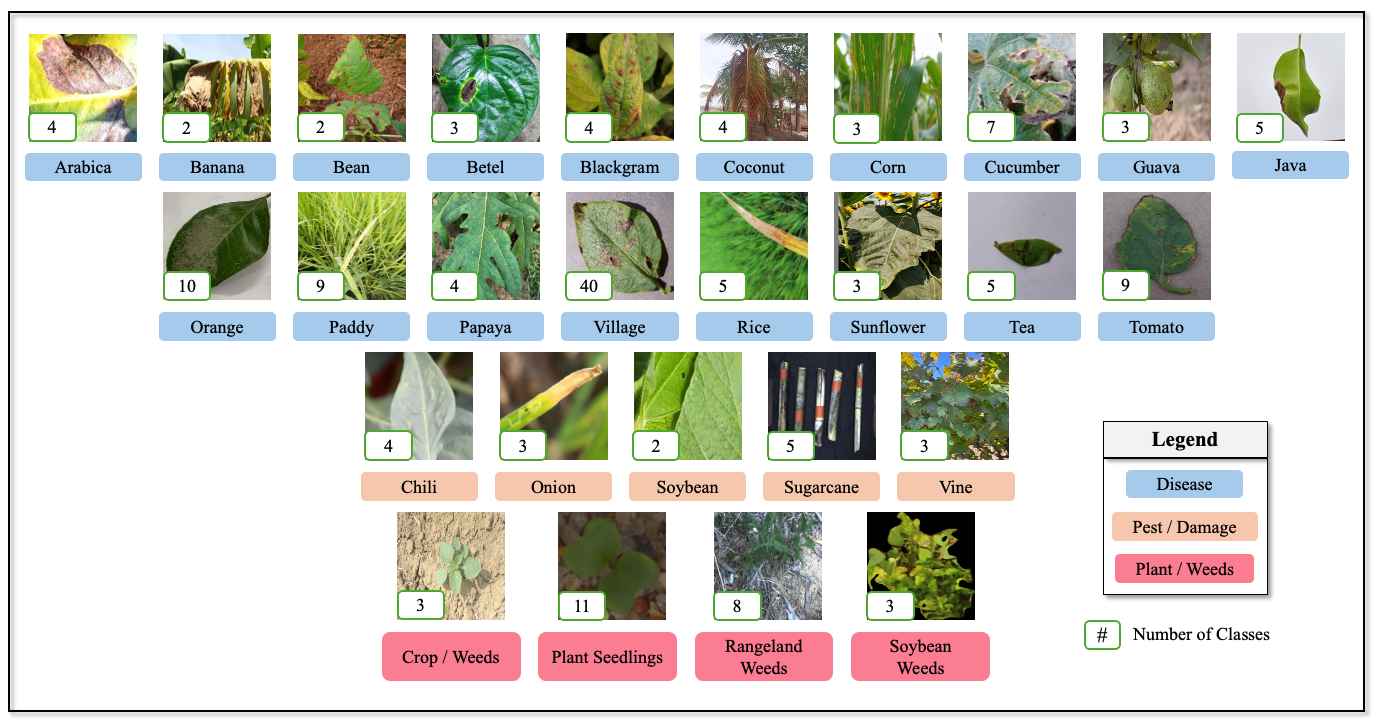
\includegraphics[width=1.0\linewidth]{dataset.png}
    \caption{Model performance was evaluated using 26 datasets spanning 121 classes from the AgML collection, totaling 248,000 images. These datasets were collected from a wide range of geographic locations and plant species. The tasks derived from these datasets include plant disease identification tasks, pest and damage detection, and plant or weed species classification.}
    \label{fig:dataset_overview}
\end{figure*}

MCQA provides a controlled, directly comparable measure of classification performance across models, while OEQ evaluates a model’s ability to produce semantically correct, unconstrained responses without reliance on predefined context, better reflecting real-world deployment conditions. Each MCQA question has a maximum for four choices.
 
Of the questions contained in the test set for MCQA 2--4, 70\% contains the correct class answer while the remaining 30\% has ``None of the above'' as the correct answer (Section~\ref{sec:prompt_methodology}). Of the NOTA samples, we omitted the ground-truth label while keeping the associated image. The fixed 30\% ``None of the above'' rate is a design choice that may not reflect the true prior probability of negative samples in real-world deployment scenarios. Since this ratio is held constant across all models and datasets, it does not differentially bias model comparisons, but future work should explore whether calibrated negative sampling rates affect absolute performance estimates. We additionally conduct a dedicated sensitivity analysis over this rate in Section~\ref{sec:prompt_sensitivity}, confirming that our reported accuracies are not an artifact of the specific 30\% choice.
 
To manage the computational overhead and API usage costs associated with evaluating large-scale commercial and open-weight VLMs (e.g., GPT-5, Gemini-3-Pro, Claude-Haiku-4.5, and Qwen-VL-72B), we employed a representative subsampling strategy during our zero-shot evaluations. Specifically, rather than utilizing the full validation split for each dataset, we evaluated a random 10\% subset of the images in the validation split. To ensure equitable comparisons, the same fixed random seed was used to draw this subset for every subsampled model, so all subsampled models are scored on the identical set of images per dataset (Supplementary Table~\ref{tab:subsample_counts}\ verifies this directly). We used stratified random sampling per class to preserve the original class distribution as closely as possible; for classes with very few images ($n \lesssim 10$), a 10\% draw can round to zero, so proportions are not always preserved exactly and a small number of classes are entirely absent from the subsample for a few datasets. We quantify and disclose this explicitly in Supplementary Section~\ref{sec:supplementary}.

\begin{figure*}[t]
    \centering
    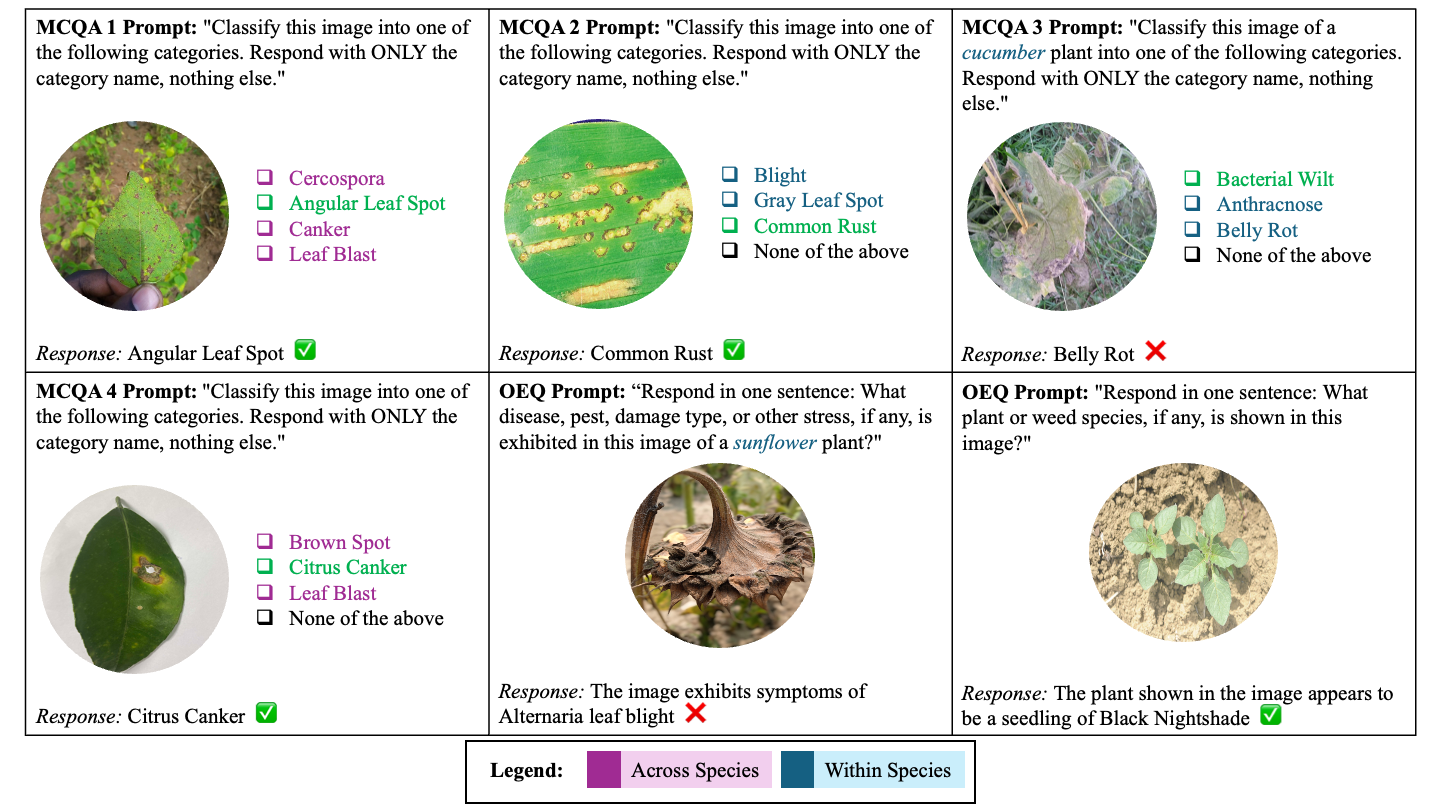
\includegraphics[width=1.0\linewidth]{prompts_overview.png}
    \caption{An overview of the evaluation prompts used. In the MCQA options,
    purple text denotes classes drawn from different species, while blue text
    indicates classes drawn from the same species. A ``None of the Above''
    option was included in MCQA~2--4 to assess whether a model can recognize
    when none of the presented options are visually present in the image.}
    \label{fig:prompts_overview}
\end{figure*}

\subsection{ICL Setup}
\label{sec:icl_setup}
For the ICL experiments, we evaluated 1-shot, 2-shot, 5-shot, and balanced-shot learning configurations to examine how the model responds under varying amounts of context. All ICL experiments were conducted using Qwen3-VL-8B (Instruct), selected as a representative open-source model capable of processing interleaved image-text inputs required for in-context demonstrations. Experiments were conducted using two prompt variants defined in Table~\ref{tab:prompts}: MCQA 3 and OEQ. Each prompt was initialized by loading the base template, then appended with the following instruction: ``Here are image and label examples of disease, pest, damage, or other stresses:'' followed by the corresponding number of image-label pairs required by each configuration. To assess the sensitivity of results to example selection, each $k$-shot configuration was repeated across five random seeds (42, 100, 123, 500, 999), and performance is reported as mean $\pm$ standard deviation across runs. For balanced sampling, rather than increasing context length, one image-label pair per class was provided to ensure full class coverage within the prompt. As such, any performance differences between 5-shot and balanced sampling reflect the effect of class coverage rather than additional context volume, and the two conditions are not directly comparable in terms of context scaling.

\subsection{Metrics}                                    
The accuracy metric is used to quantify model performance using two complementary approaches: exact match accuracy (based on fuzzy string matching) and LLM judge accuracy (based on semantic evaluation). For a dataset of $N$ samples with ground-truth labels $y_i$ and predicted labels $\hat{y}_i$, accuracy is computed as the proportion of correct predictions:

\begin{equation}
  \text{Accuracy} = \frac{1}{N} \sum_{i=1}^{N} \mathbf{1}[\hat{y}_i = y_i]
\end{equation}

\noindent where $\mathbf{1}[\cdot]$ is the indicator function. The macro-averaged F1-score was also computed to account for class imbalance across datasets:

\begin{equation}                                          
  F1 = \frac{2 \cdot \text{Precision} \cdot \text{Recall}}{\text{Precision} + \text{Recall}}
\end{equation}

\noindent where $\text{Precision} = TP / (TP + FP)$ and $\text{Recall} = TP / (TP + FN)$ are computed per class and averaged across all classes (macro-average) to treat each class equally regardless of sample size.

A naive baseline accuracy is also reported, representing a model that always predicts the most frequent class in each dataset:

\begin{equation}                                          
  \text{Accuracy}_{\text{naive}} = \frac{\max_{c \in \mathcal{C}} |S_c|}{|S|}
\end{equation}

\noindent where $\mathcal{C}$ is the set of all classes, $S$ is the full evaluation set, and $|S_c|$ is the number of samples belonging to class $c$. This provides a lower-bound reference point reflecting the performance achievable by always predicting the majority class.

\begin{figure*}[t]
    \centering
    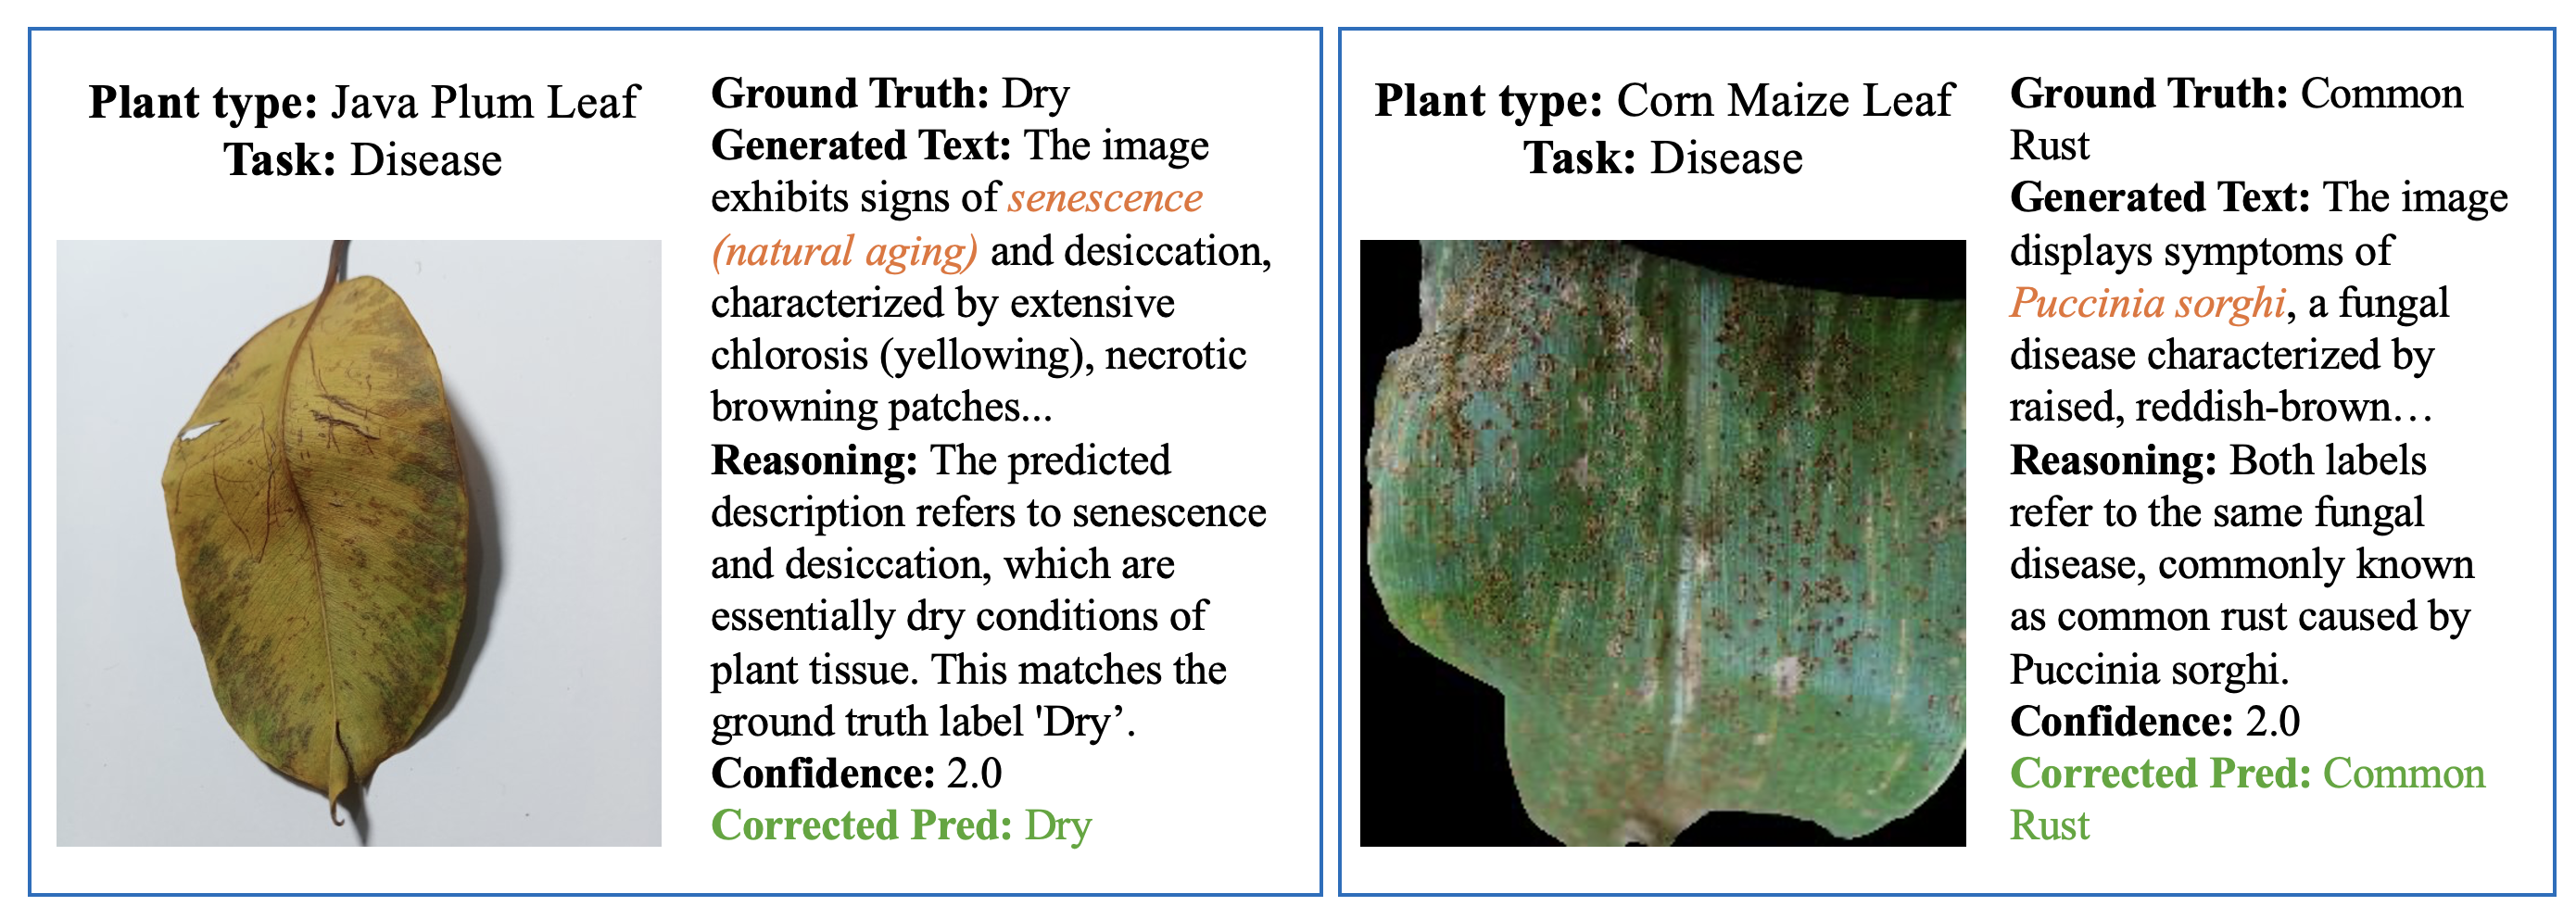
\includegraphics[width=0.8\linewidth]{judge_samples.png}
    \caption{Sample LLM judge assessments, using OpenAI's GPT-OSS-20B model,
    showing that the predicted class (orange) and the ground truth label are
    the same. The corrected prediction is shown in green.}
    \label{fig:judge_samples}
\end{figure*}

\begin{figure}[t]
    \centering
    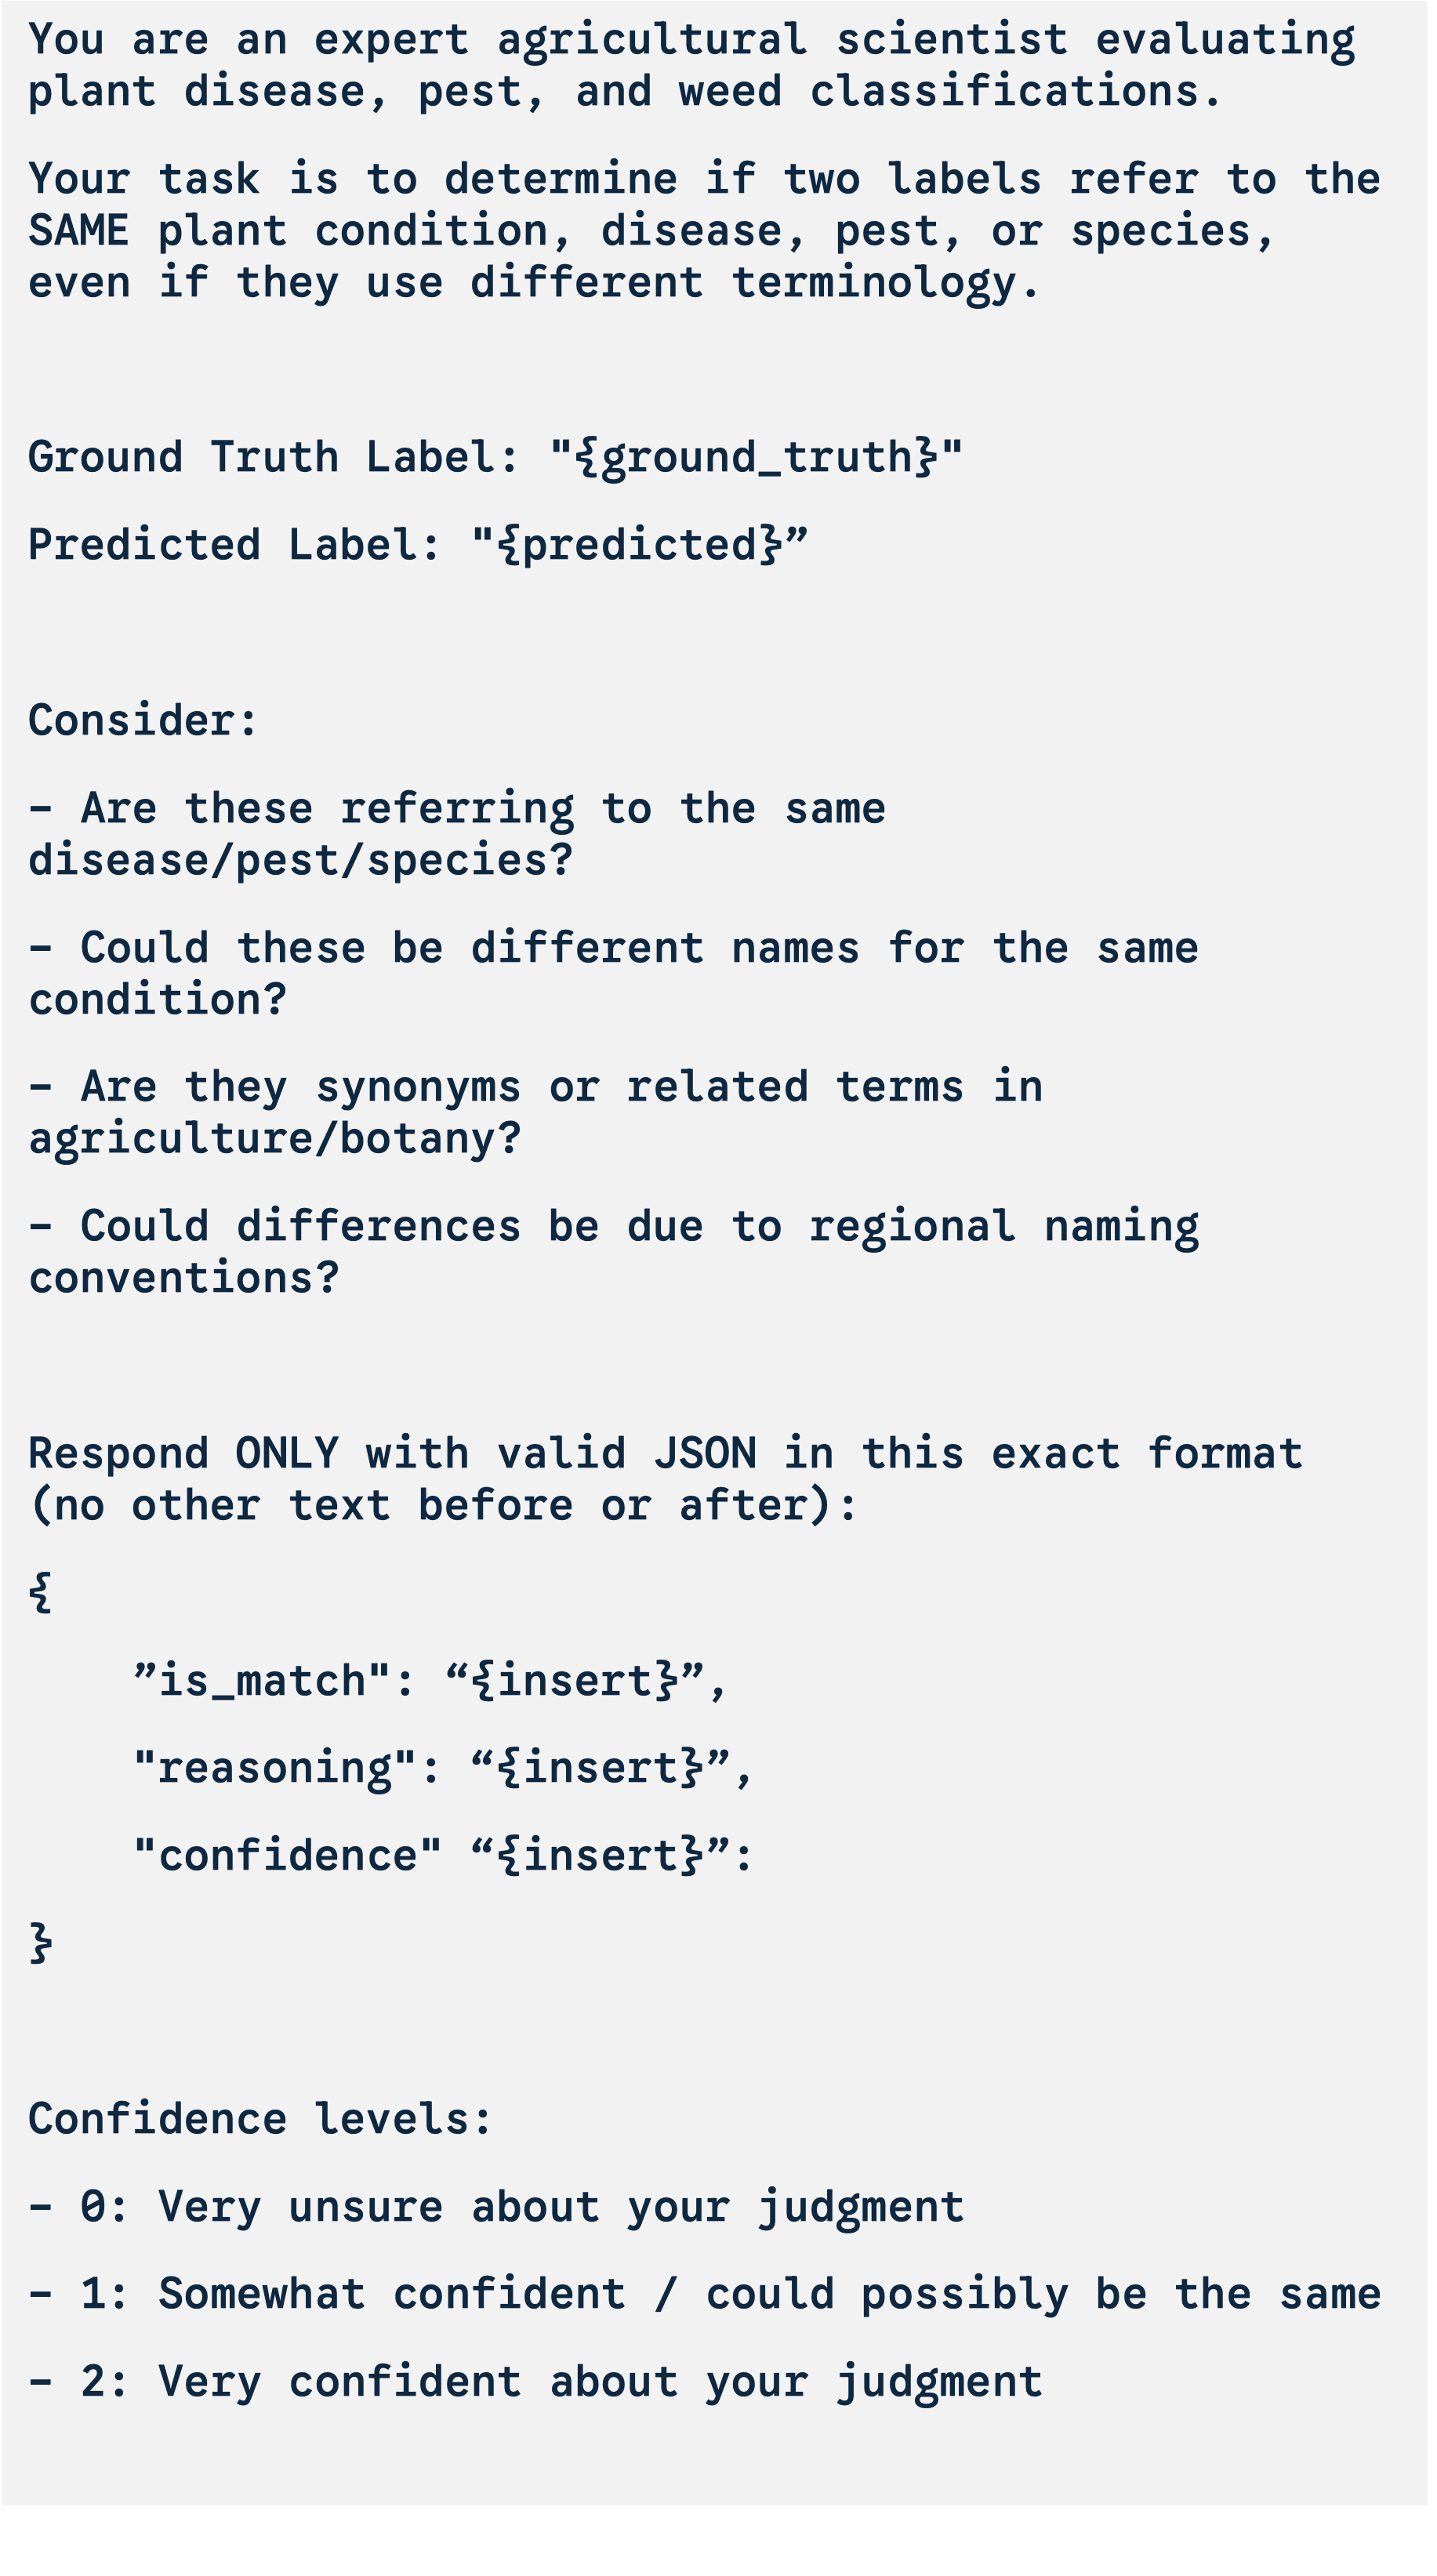
\includegraphics[width=0.4\linewidth]{judge_prompt.png}
    \caption{LLM judge prompt to frame the task as a semantic assessment in an
    agricultural context. The prompt explicitly instructs the judge to consider
    agricultural domain knowledge and to output a JSON structure containing
    three fields: \texttt{is\_match} (boolean indicating equivalence),
    \texttt{reasoning} (brief explanation of the judgment), and
    \texttt{confidence} (0-2 integer scale). The confidence scale enables
    thresholding which allows us to adjust the strictness of the judge.}
    \label{fig:judge_prompt}
\end{figure}

For exact match accuracy, model-generated text responses are matched to ground-truth labels using a multi-stage fuzzy string matching algorithm. First, the generated text undergoes preprocessing: conversion to lowercase, removal of common model-added prefixes (e.g., "the answer is", "category:"), and removal of trailing punctuation. Then, three matching stages are applied in order: (1) exact string match after preprocessing, (2) substring containment check, and (3) fuzzy matching if neither exact nor substring matches are found. For fuzzy matching, two similarity measures are computed: character-level sequence similarity (using Python's SequenceMatcher) and word overlap ratio (proportion of label tokens found in the generated text). The maximum of these two scores is used as the final similarity score. Predictions are considered correct only if the similarity score is greater than or equal to 0.6 (60\%). The 0.6 threshold was explicitly utilized as a preliminary, conservative pre-filter to catch obvious exact matches. It does not serve as the final arbiter of correctness for complex generation. This approach handles the inherent variability in free-form VLM responses where models may include alternative phrasing or additional context beyond the exact class name.

\begin{table*}[ht]
\centering
\caption{Model performance by task category (OEQ results are derived from fuzzy match results). Accuracy (\%) and macro-averaged F1-score are reported as mean $\pm$ standard deviation across datasets. Overall Avg.\ is the unweighted mean across the three task categories. (*) indicates models evaluated on a 10\% stratified subsample for cost efficiency; GPT-5-Nano was evaluated on the full validation split and is unmarked. SFT = supervised fine-tuning.}
\label{tab:main_results}
\renewcommand{\arraystretch}{1.2}
\resizebox{\textwidth}{!}{%
\begin{tabular}{llcccccccc}
\toprule
\multirow{2}{*}{\textbf{Method}} & \multirow{2}{*}{\textbf{Model}}
    & \multicolumn{2}{c}{\textbf{Overall Avg.}}
    & \multicolumn{2}{c}{\textbf{Disease} ($n=17$)}
    & \multicolumn{2}{c}{\textbf{Pest/Damage} ($n=5$)}
    & \multicolumn{2}{c}{\textbf{Plant/Weeds} ($n=4$)} \\
\cmidrule(lr){3-4} \cmidrule(lr){5-6} \cmidrule(lr){7-8} \cmidrule(lr){9-10}
& & Acc. (\%) & F1
  & Acc. (\%) & F1
  & Acc. (\%) & F1
  & Acc. (\%) & F1 \\
\midrule
\multirow{2}{*}{Each dataset}
    & YOLO11 (SFT)
        & $\mathbf{97.82}$ & $\mathbf{0.97}$
        & $97.79 \pm 4.07$  & $0.98 \pm 0.04$
        & $96.81 \pm 3.18$  & $0.95 \pm 0.06$
        & $98.85 \pm 1.14$  & $0.99 \pm 0.01$ \\
    & Naive Baseline
        & $0.33$ & ---
        & $0.26$ & ---
        & $0.35$ & ---
        & $0.38$ & --- \\
\midrule
\multirow{10}{*}{MCQA 1}
    & SigLIP2
        & $30.18$ & $0.21$
        & $24.88 \pm 15.36$ & $0.16 \pm 0.14$
        & $23.94 \pm  7.26$ & $0.11 \pm 0.05$
        & $41.72 \pm 33.87$ & $0.36 \pm 0.33$ \\
    & LLaVA-NeXT-8B
        & $19.08$ & $0.07$
        & $18.60 \pm  8.52$ & $0.07 \pm 0.05$
        & $27.63 \pm 14.33$ & $0.11 \pm 0.07$
        & $11.01 \pm  8.89$ & $0.04 \pm 0.04$ \\
    & Qwen2.5-VL-7B
        & $43.51$ & $0.36$
        & $46.64 \pm 21.83$ & $0.40 \pm 0.23$
        & $34.61 \pm 21.76$ & $0.27 \pm 0.21$
        & $49.28 \pm 30.79$ & $0.42 \pm 0.32$ \\
    & Gemma-3-4B
        & $34.08$ & $0.27$
        & $40.61 \pm 15.90$ & $0.35 \pm 0.17$
        & $32.95 \pm 14.81$ & $0.24 \pm 0.11$
        & $28.67 \pm 21.66$ & $0.21 \pm 0.15$ \\
    & Deepseek-VL-7B
        & $34.41$ & $0.26$
        & $39.50 \pm 18.68$ & $0.32 \pm 0.20$
        & $31.47 \pm 12.01$ & $0.19 \pm 0.11$
        & $32.26 \pm 19.57$ & $0.27 \pm 0.19$ \\
    & Qwen2.5-VL-72B*
        & $41.36$ & $0.34$
        & $48.14 \pm 21.95$ & $0.42 \pm 0.25$
        & $39.06 \pm 16.35$ & $0.29 \pm 0.15$
        & $36.87 \pm 12.41$ & $0.32 \pm 0.19$ \\
    & GPT-5-Nano
        & $39.38$ & $0.33$
        & $49.10 \pm 19.78$ & $0.44 \pm 0.21$
        & $40.35 \pm 21.21$ & $0.30 \pm 0.19$
        & $28.69 \pm 22.68$ & $0.24 \pm 0.22$ \\
    & GPT-5*
        & $53.98$ & $0.47$
        & $60.67 \pm 18.54$ & $0.57 \pm 0.21$
        & $50.16 \pm 15.17$ & $0.39 \pm 0.15$
        & $51.11 \pm 36.95$ & $0.45 \pm 0.40$ \\
    & Gemini-3 Pro*
        & $\mathbf{61.78}$ & $\mathbf{0.47}$
        & $\mathbf{61.76} \pm 16.24$ & $\mathbf{0.54} \pm 0.17$
        & $\mathbf{49.72} \pm 14.29$ & $\mathbf{0.33} \pm 0.14$
        & $\mathbf{73.87} \pm 13.35$ & $\mathbf{0.55} \pm 0.08$ \\
    & Claude Haiku 4.5*
        & $34.13$ & $0.27$
        & $39.82 \pm 21.27$ & $0.33 \pm 0.19$
        & $30.36 \pm 23.97$ & $0.22 \pm 0.15$
        & $32.22 \pm 20.49$ & $0.25 \pm 0.20$ \\
\midrule
\multirow{9}{*}{\shortstack[l]{Zero-shot \\ OEQ}}
    & LLaVA-NeXT-8B
        & $ 2.07$ & $0.02$
        & $ 2.28 \pm  2.88$ & $0.03 \pm 0.04$
        & $ 2.98 \pm  3.89$ & $0.03 \pm 0.04$
        & $ 0.96 \pm  1.35$ & $0.01 \pm 0.02$ \\
    & Qwen2.5-VL-7B
        & $ 2.45$ & $0.03$
        & $ 1.81 \pm  6.02$ & $0.02 \pm 0.05$
        & $ 0.04 \pm  0.07$ & $0.00 \pm 0.00$
        & $ 5.51 \pm  9.03$ & $0.07 \pm 0.10$ \\
    & Gemma-3-4B
        & $ 6.46$ & $0.06$
        & $ 4.28 \pm  5.65$ & $0.03 \pm 0.03$
        & $ 6.61 \pm 11.06$ & $0.05 \pm 0.07$
        & $ 8.49 \pm 10.60$ & $0.09 \pm 0.11$ \\
    & Deepseek-VL-7B
        & $ 3.66$ & $0.03$
        & $ 0.17 \pm  0.36$ & $0.00 \pm 0.01$
        & $ 0.08 \pm  0.08$ & $0.00 \pm 0.00$
        & $10.72 \pm 12.72$ & $0.08 \pm 0.10$ \\
    & Qwen2.5-VL-72B*
        & $17.92$ & $0.14$
        & $16.29 \pm 19.08$ & $0.16 \pm 0.18$
        & $14.78 \pm  6.76$ & $0.14 \pm 0.03$
        & $22.70 \pm 28.18$ & $0.12 \pm 0.13$ \\
    & GPT-5-Nano
        & $12.55$ & $0.11$
        & $15.51 \pm 16.56$ & $0.14 \pm 0.13$
        & $ 8.54 \pm  8.29$ & $0.08 \pm 0.08$
        & $13.60 \pm 16.38$ & $0.11 \pm 0.12$ \\
    & GPT-5*
        & $\mathbf{20.80}$ & $\mathbf{0.20}$
        & $\mathbf{24.89} \pm 18.68$ & $\mathbf{0.23} \pm 0.15$
        & $\mathbf{13.53} \pm 13.98$ & $\mathbf{0.14} \pm 0.14$
        & $23.98 \pm 21.67$ & $0.22 \pm 0.12$ \\
    & Gemini-3 Pro*
        & $20.31$ & $0.16$
        & $17.18 \pm 14.07$ & $0.15 \pm 0.11$
        & $11.92 \pm 10.76$ & $0.11 \pm 0.09$
        & $\mathbf{31.84} \pm 32.17$ & $\mathbf{0.23} \pm 0.17$ \\
    & Claude Haiku 4.5*
        & $ 5.52$ & $0.05$
        & $10.22 \pm  7.45$ & $0.09 \pm 0.07$
        & $ 2.36 \pm  2.21$ & $0.03 \pm 0.03$
        & $ 3.97 \pm  4.88$ & $0.04 \pm 0.04$ \\
\bottomrule
\end{tabular}%
}
\end{table*}

\subsection{LLM Judging}
\label{sec:llm_judging}
Fuzzy matching has limitations as it may fail to recognize semantically equivalent labels with different terminology such as: “leaf blight” vs.  “leaf spot”. Conversely, “early blight” and “late blight” have high textual similarity but refer to entirely different conditions. To capture semantic correctness beyond surface-level text matching, we use a LLM, the judge model, to evaluate whether predictions and ground truth labels refer to the same thing, even when phrased differently. In this case, we use OpenAI’s GPT-OSS-20B model \cite{openai_gpt-oss-120b_2025} with reasoning capabilities. The judge evaluates each prediction using a designed prompt that frames the task as a semantic assessment in an agricultural context, shown in Figure \ref{fig:judge_samples} and \ref{fig:judge_prompt}.

The prompt explicitly instructs the judge to consider agricultural domain knowledge and to output a JSON structure containing three fields: \texttt{is\_match} (boolean indicating equivalence), \texttt{reasoning} (brief explanation of the judgement), and \texttt{confidence} (0-2 integer scale). The confidence scale enables thresholding which allows us to adjust the strictness of the judge. In this experiment, we only kept scores with confidence scores of 2 (high confidence that the predicted response matches the ground-truth label).

To validate the LLM judge, a human reviewer manually inspected up to 10 judge decisions per dataset where the judge and fuzzy string matching disagreed, sampling both false positives (judge marked a correct prediction as wrong) and false negatives (judge marked a wrong prediction as correct). This auditing was performed on the
predictions of two representative models, the best-performing open-source model (Qwen-VL-72B) and the best-performing closed-source model (Gemini-3 Pro), separately for each task category (disease, pest/damage, and plant/weed species). Judge reliability per task was quantified using the audited edge-case agreement rate:

\begin{equation}
    \text{Accuracy}_{\text{audit}} = \frac{N_{\text{agreements}}}{N_{\text{audited}}}
\end{equation}

\noindent where $N_{\text{audited}}$ is the number of ambiguous mismatch cases manually reviewed per task, and $N_{\text{agreements}}$ is the number of those cases where the human reviewer confirmed the judge's verdict. This metric was computed separately for each task (disease, pest/damage, and plant/weed species).

\begin{figure*}[h]
    \centering
    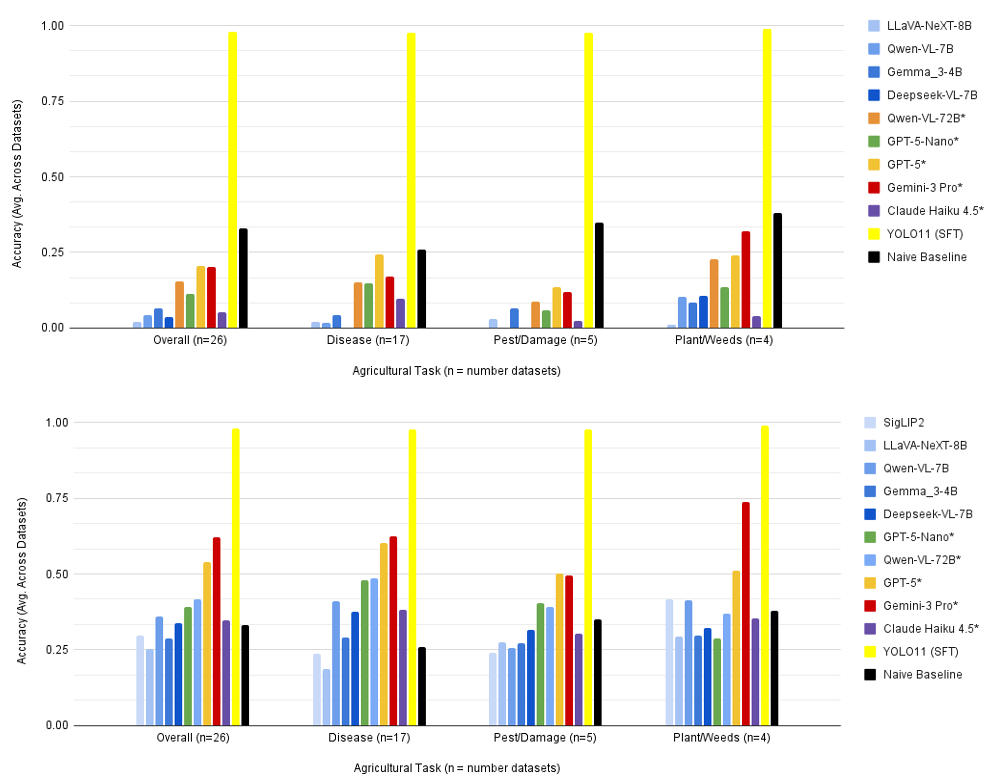
\includegraphics[width=0.9\linewidth]{main_results.png}
    \caption{OEQ (top) and MCQA~1 (bottom) results (OEQ results are derived from fuzzy match results). Accuracy is averaged across datasets for each classification task, with overall accuracy computed across disease, pest/damage, and weed classification. (*) indicates models evaluated on a reduced validation subset for cost efficiency. We define $n$ as the number of datasets used for each task.}
    \label{fig:main_results_chart}
\end{figure*}

\begin{figure*}[h]
    \centering
    \begin{minipage}{0.45\linewidth}
        \centering
        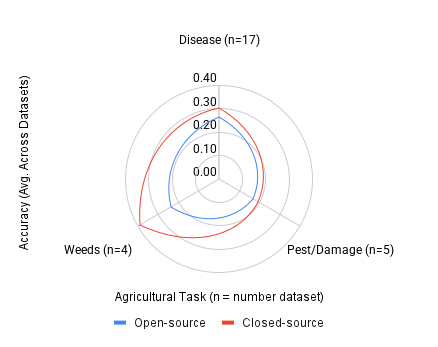
\includegraphics[width=\linewidth]{best_open_closed.png}
    \end{minipage}
    \hfill
    \begin{minipage}{0.48\linewidth}
        \centering
        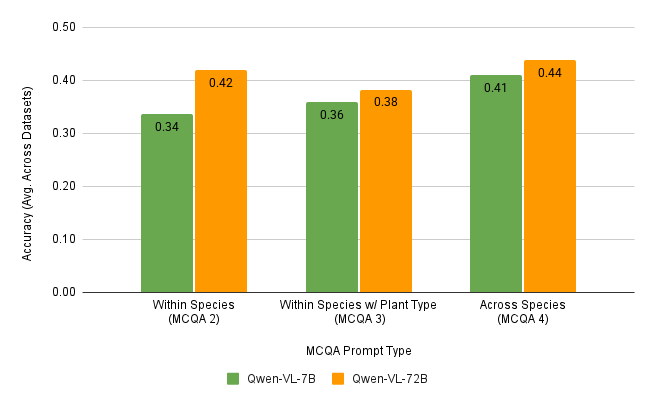
\includegraphics[width=\linewidth]{mcqa_comp.png}
    \end{minipage}
    \caption{(Left) Best performing closed-source model, Gemini-3 Pro, and best performing open-source model, Qwen2.5-VL-72B from OEQ judged results. (Right) MCQA results with ``None of the above'' included as an option. MCQA~2 and 3 include classes within species. MCQA~4 includes classes across species.}
    \label{fig:judge_and_best}
\end{figure*}

\begin{table*}[t]
\centering
\caption{OEQ judged accuracy results by task category for Gemini-3-Pro (closed-source) and Qwen2.5-VL-72B (open-source). Judged Accuracy delta represents the gain over exact-match accuracy when using LLM-based semantic evaluation. Judge Validation is the human-verified agreement rate on audited mismatch cases.}
\label{tab:judge_val}
\renewcommand{\arraystretch}{1.2}
\resizebox{\textwidth}{!}{%
\begin{tabular}{lcccccccccccc}
\toprule
\multirow{2}{*}{\textbf{Model}}
    & \multicolumn{3}{c}{\textbf{Overall Avg.}}
    & \multicolumn{3}{c}{\textbf{Disease}}
    & \multicolumn{3}{c}{\textbf{Pest/Damage}}
    & \multicolumn{3}{c}{\textbf{Plants/Weeds}} \\
\cmidrule(lr){2-4} \cmidrule(lr){5-7} \cmidrule(lr){8-10} \cmidrule(lr){11-13}
    & Acc. & $\Delta$Judge & Val.
    & Acc. & $\Delta$Judge & Val.
    & Acc. & $\Delta$Judge & Val.
    & Acc. & $\Delta$Judge & Val. \\
\midrule
Naive Baseline
    & 0.33 & --- & ---
    & 0.26 & --- & ---
    & 0.35 & --- & ---
    & 0.38 & --- & --- \\
\midrule
Qwen2.5-VL-72B
    & 0.22 & $+$0.07 & 0.87
    & 0.26 & $+$0.11 & 0.88
    & 0.17 & $+$0.08 & 0.93
    & 0.24 & $+$0.01 & 0.80 \\
Gemini-3 Pro*
    & 0.30 & $+$0.11 & 0.87
    & 0.31 & $+$0.14 & 0.87
    & 0.19 & $+$0.07 & 1.00
    & 0.39 & $+$0.13 & 0.63 \\
\bottomrule
\end{tabular}%
}
\end{table*}

\begin{figure}[ht]
    \centering
    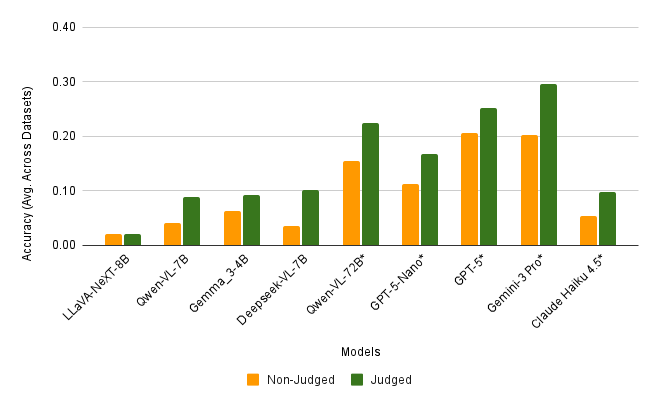
\includegraphics[width=0.8\linewidth]{judge_results.png}
    \caption{LLM judge results for all models evaluated using the OEQ setting.
    Full judged accuracy values for all models are shown here;
    Table~\ref{tab:judge_val} reports detailed per-task breakdowns and human
    validation rates for the two representative models.}
    \label{fig:judge_results_chart}
\end{figure}

\begin{table}[t]
\centering
\caption{In-context learning results for Qwen3-VL-8B (Instruct) across MCQA~3 and OEQ prompt variants. Baseline ($k=0$) is zero-shot with no in-context examples. For $k \geq 1$, results are reported as mean $\pm$ standard deviation across five random seeds (42, 100, 123, 500, 999). Balanced sampling provides one image-label pair per class and is not directly comparable to $k$-shot configurations in terms of context scaling.}
\label{tab:icl_results}
\renewcommand{\arraystretch}{1.2}
\footnotesize
\begin{tabular}{lcc}
\toprule
& \multicolumn{2}{c}{\textbf{Overall Avg. Accuracy}} \\
\cmidrule(lr){2-3}
\textbf{$k$} & \textbf{MCQA 3} & \textbf{OEQ} \\
\midrule
0             & 0.40            & 0.13 \\
1             & $0.44 \pm 0.08$ & $0.25 \pm 0.02$ \\
2             & $0.46 \pm 0.05$ & $0.31 \pm 0.04$ \\
5             & $0.52 \pm 0.04$ & $0.42 \pm 0.05$ \\
balanced      & $0.48 \pm 0.04$ & $0.42 \pm 0.05$ \\
\bottomrule
\end{tabular}
\end{table}


\section{Results}
\label{sec:results}

\subsection{Zero-shot Results}
As expected, the supervised YOLO11 model substantially outperformed all zero-shot vision-language models, achieving over 95\% accuracy across all three task categories. Among foundation models evaluated under MCQA 1 prompting, summarized in Table~\ref{tab:main_results} and Figure~\ref{fig:main_results_chart}, Gemini-3 Pro achieved the highest overall average accuracy at 62\%, consistently outperforming all other models across each individual task. Paired bootstrap resampling (10,000 iterations) confirmed this gap is statistically significant; the 12.7pp difference between Gemini-3 Pro (68.6\%) and GPT-5 (56.0\%) across all 26 datasets yields a 95\% CI of [+11.1, +14.2]pp ($p < 0.001$), with 9 of 26 individual datasets reaching significance independently.

In the zero-shot OEQ setting, GPT-5 attained the highest overall average raw accuracy at 21\%, though all models remained below the naive baseline. When evaluated using LLM-based semantic judging, Gemini-3 Pro emerged as the top OEQ performer at 30\%, followed by GPT-5 at 25\%, as displayed in Figure~\ref{fig:judge_results_chart}. Despite this improvement, judged accuracy still did not exceed the naive baseline overall, largely driven by consistently low performance on pest and damage identification, as seen from the validated judge results in Table~\ref{tab:judge_val}.

Overall, open-source models consistently underperformed relative to their closed-source counterparts. The largest open-source model evaluated, Qwen2.5-VL-72B, was the strongest among open-source models and approached the performance of some closed-source systems, likely attributable to its substantially larger parameter count. Qwen2.5-VL-72B achieved an overall accuracy of 41\% under MCQA prompting and a judged OEQ accuracy of 22\%.

Performance varied substantially across datasets, as reflected by the large standard deviations reported in Table~\ref{tab:main_results}. For example, under MCQA 1 prompting, Gemini-3 Pro achieved a standard deviation of 16\% on disease classification and 13\% on plant and weed species, indicating that model performance is highly sensitive to the specific dataset evaluated. Given this dataset-level variability, differences in accuracy of less than $\sim$5 percentage points between models should be interpreted with caution and may not reflect statistically reliable performance gaps.

Subsampling at 10\% was applied exclusively to closed-source API models and Qwen2.5-VL-72B to reduce inference costs, while all other open-source models were evaluated on the full dataset. To validate this strategy, we ran Qwen2.5-VL-72B on both the full dataset (acc. = 43.4\%) and a 10\% stratified subsample across 4 random seeds (mean = 44.4\% $\pm$ 0.9\%, CV = 2.0\%). The 0.9\% difference between the subsample estimate and the full dataset falls within the seed variance, confirming the subsample is a reliable proxy for full-dataset performance. Relative rankings among closed-source models are stable across seeds (CV = 2.0\%), supporting the validity of this evaluation strategy for cost-constrained API models. Paired bootstrap resampling additionally confirms the best-open vs.\ best-closed-source gap is statistically robust under this evaluation protocol: Gemini-3 Pro (67.9\%) outperforms Qwen2.5-VL-72B (48.7\%) by 19.2pp across the 19 datasets with predictions available for both models (95\% CI [+17.3, +21.1]pp, $p < 0.001$, 13 of 19 datasets individually significant). Supplementary Section~\ref{sec:supplementary}\ reports the exact per-dataset image counts after subsampling and confirms that every subsampled model shares the identical drawn subset for each dataset.

Based on the 60\% similarity score threshold, we report FP rates for MCQA settings 1-4 respectively: 0.17\%, 2.55\%, 0.11\%, and 2.33\%. The majority of these cases reflect model prediction errors (the model named the wrong class) rather than threshold-induced confusions between similar class names.

\subsection{Task Comparisons}
At the task level, shown on the left of Figure~\ref{fig:judge_and_best}, Gemini-3 Pro achieved its strongest OEQ judged performance on plant and weed species identification at 39\%, compared to 31\% for disease and 19\% for pest/damage classification. This pattern was broadly consistent across most models: pest and damage identification was the most challenging task, while plant and weed species classification generally yielded the highest accuracy. These task-level differences were most pronounced among 
closed-source models.

As shown on the right of Figure \ref{fig:judge_and_best}, Qwen2.5-VL-7B and Qwen2.5-VL-72B performed best on MCQA 3 (42\% and 45\%, respectively). This suggests that including cross-species distractors inflates accuracy, while restricting options to the target species yields lower, and likely more realistic, performance estimates.

\subsection{Judge Validation}
The LLM judge consistently assigned higher accuracy than fuzzy string matching across both models and all task categories, as reflected by the positive $\Delta$Judge values in Table~\ref{tab:judge_val}. The largest gains were observed for disease classification, where Qwen2.5-VL-72B and Gemini-3 Pro improved by $+$0.11 and $+$0.14, respectively. In contrast, the smallest delta was observed for plant and weed species in Qwen2.5-VL-72B ($+$0.01). Judge validation accuracy was high for disease (0.88 and 0.87 for Qwen2.5-VL-72B and Gemini-3 Pro respectively) and pest/damage tasks (0.93 and 1.00) respectively, but was notably lower for plant and weed species classification (0.80 and 0.63), as shown in Table~\ref{tab:judge_val}.

\subsection{ICL Results}
For the MCQA 3 and OEQ prompt variants, model accuracy improved consistently with the number of $k$-shot context samples, as shown in Table~\ref{tab:icl_results}. MCQA 3 showed increasing overall accuracy from 40\% at baseline to 44\% at 1-shot and 52\% at 5-shot. OEQ displayed similar trends, rising from 13\% at baseline to 42\% at 5-shot. Under balanced sampling, MCQA 3 achieved 48\% and OEQ reached 42\%, compared to 52\% and 42\% at 5-shot, respectively.

\subsection{Prompt Sensitivity Ablation}
\label{sec:prompt_sensitivity}

We conducted a dedicated prompt-sensitivity ablation study to test whether our central conclusions, the superiority of MCQA over open-ended prompting, and the role of species-level cues, are robust to specific choices in prompt wording rather than artifacts of the particular templates used in Table~\ref{tab:prompts}. Because exhaustively crossing every prompt dimension is computationally infeasible at the scale of our benchmark (26 datasets $\times$ multiple prompt families), we prioritize three ablations most directly tied to these claims: (1) randomization of MCQA answer order, (2) sensitivity to the ``None of the above'' rejection rate, and (3) common vs.\ scientific species names in both MCQA and OEQ prompts. We run each ablation across all applicable datasets on two representative open-source models, Qwen2.5-VL-7B and Gemma-3-4B, and report results aggregated by task group (disease, pest/damage, weeds) with variability, so the reader can see the spread rather than a single point estimate.

\begin{table}[t]
\centering
\caption{Answer-order randomization ablation (Section~\ref{sec:prompt_sensitivity}): MCQA~2 accuracy (\%) under five independently seeded random option orderings, with the position of ``None of the above'' also randomized. Reported as mean $\pm$ std.\ across the five orderings, averaged over datasets within each task group.}
\label{tab:ablation_order}
\renewcommand{\arraystretch}{1.2}
\footnotesize
\begin{tabular}{lcc}
\toprule
\textbf{Task group} & \textbf{Gemma-3-4B} & \textbf{Qwen2.5-VL-7B} \\
\midrule
Disease & $36.6 \pm 0.6$ & $39.7 \pm 0.3$ \\
Pest/Damage & $29.7 \pm 2.5$ & $27.9 \pm 1.0$ \\
Weeds & $32.1 \pm 0.9$ & $39.0 \pm 1.3$ \\
\bottomrule
\end{tabular}
\end{table}

\textbf{Answer-order randomization.} For each MCQA~2 sample, we regenerate the option list under five independently seeded random orderings, with the position of ``None of the above'' also randomized rather than fixed at the end of the list. As shown in Table~\ref{tab:ablation_order}, accuracy varies by at most 2.5 percentage points (std.\ across the five orderings) across all task groups and both models, well within the $\sim$5pp threshold we identify elsewhere (Section~\ref{sec:results}) as attributable to dataset-level variability rather than a reliable performance gap. This indicates that our MCQA results are not an artifact of a particular option layout.

\begin{table}[t]
\centering
\caption{``None of the above'' (NOTA) rate sensitivity ablation (Section~\ref{sec:prompt_sensitivity}): MCQA~2 accuracy (\%) as the NOTA rejection rate is varied over $\{10\%, 30\%, 50\%\}$, holding the prompt otherwise fixed. Reported as mean $\pm$ std.\ across datasets within each task group. The manuscript uses 30\% throughout (Section~\ref{sec:experiment}).}
\label{tab:ablation_nota}
\renewcommand{\arraystretch}{1.2}
\footnotesize
\begin{tabular}{llccc}
\toprule
\textbf{Model} & \textbf{Task group} & \textbf{10\%} & \textbf{30\%} & \textbf{50\%} \\
\midrule
\multirow{3}{*}{Gemma-3-4B}
    & Disease & $39.8 \pm 12.7$ & $37.0 \pm 10.4$ & $34.2 \pm 9.8$ \\
    & Pest/Damage & $35.5 \pm 9.2$ & $31.3 \pm 6.7$ & $28.2 \pm 4.5$ \\
    & Weeds & $34.8 \pm 15.6$ & $32.2 \pm 11.5$ & $28.0 \pm 6.1$ \\
\midrule
\multirow{3}{*}{Qwen2.5-VL-7B}
    & Disease & $42.9 \pm 15.8$ & $40.3 \pm 13.2$ & $38.3 \pm 11.1$ \\
    & Pest/Damage & $29.3 \pm 15.0$ & $29.8 \pm 10.8$ & $28.7 \pm 9.5$ \\
    & Weeds & $37.8 \pm 19.2$ & $40.3 \pm 13.4$ & $42.2 \pm 8.2$ \\
\bottomrule
\end{tabular}
\end{table}

\textbf{``None of the above'' rate sensitivity.} We sweep the NOTA rejection rate over $\{10\%, 30\%, 50\%\}$ while holding the prompt otherwise fixed (Table~\ref{tab:ablation_nota}). Accuracy decreases modestly and consistently as the rejection rate increases for five of the six model/task-group combinations tested, by 0.6--7.3pp between the 10\% and 50\% conditions, consistent with the expectation that abstention becomes harder to calibrate as its base rate rises; the exception is Qwen2.5-VL-7B on weeds classification, where accuracy instead increases by 4.4pp. In all cases, the 30\% rate used throughout the manuscript falls between the two tested extremes rather than at either boundary, and the observed shifts are comparable in magnitude to the dataset-level variability already characterized in Section~\ref{sec:results}. We therefore conclude that our reported accuracies are not an artifact of the specific 30\% design choice, though absolute accuracy is sensitive to this rate, and we recommend that future deployments calibrate it to the true prior probability of ``no applicable label'' in their target setting.

\begin{figure}[t]
    \centering
    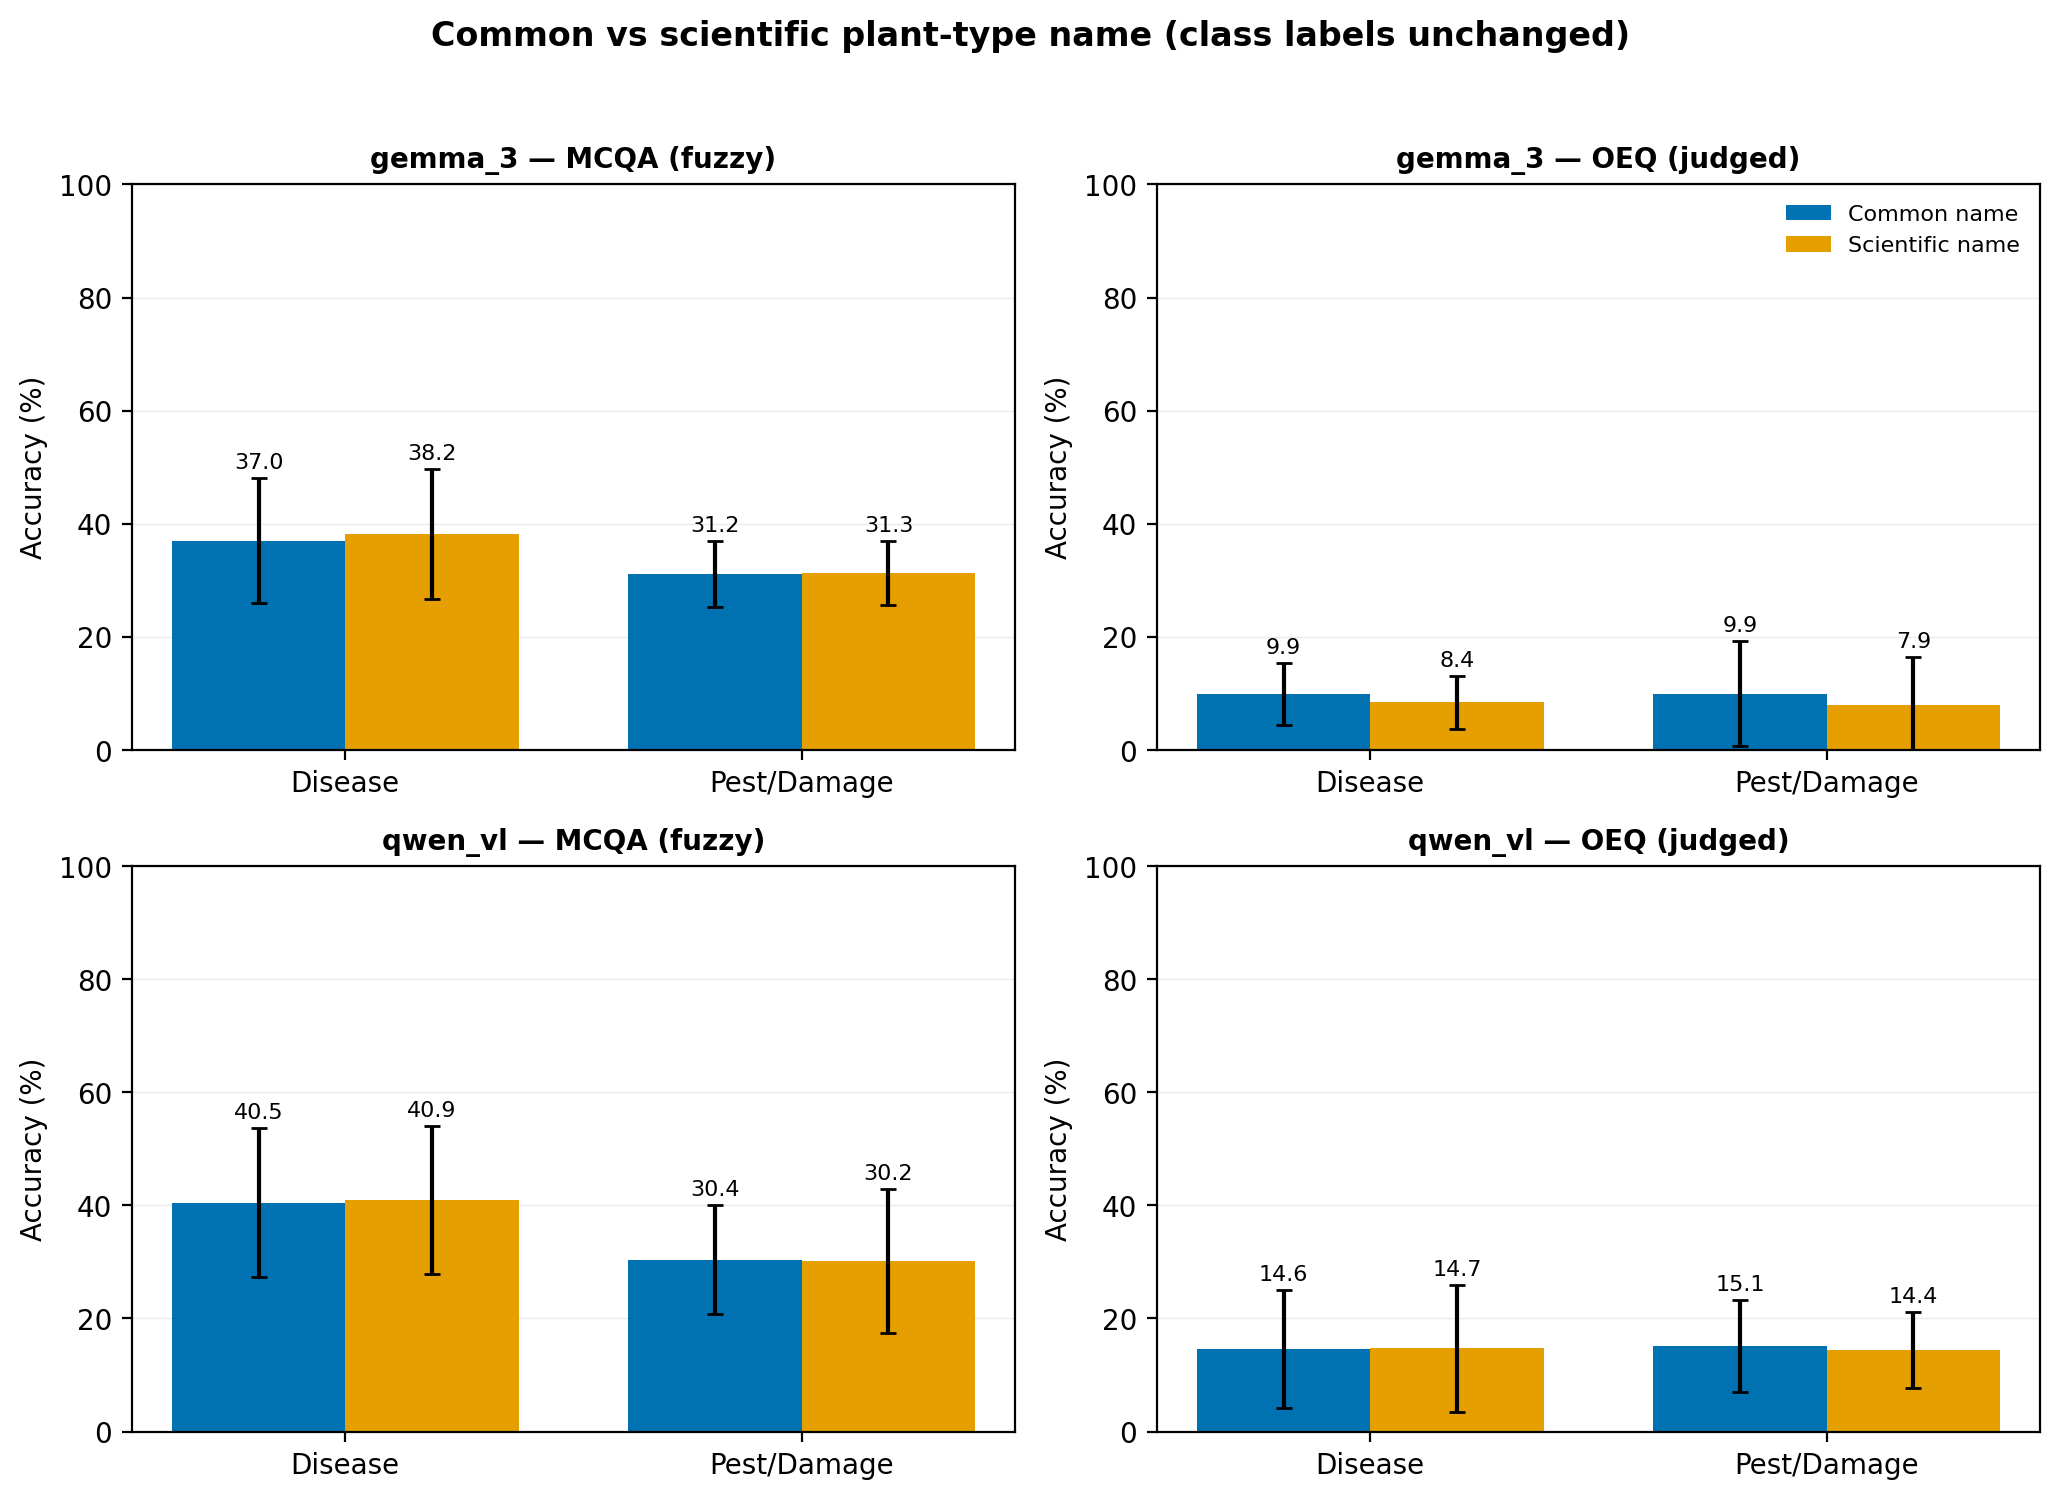
\includegraphics[width=\linewidth]{ablation_species_names.png}
    \caption{Common vs.\ scientific plant-type naming ablation (Section~\ref{sec:prompt_sensitivity}): accuracy by task group for MCQA~3 (fuzzy match) and OEQ (LLM-judged), for Gemma-3-4B and Qwen2.5-VL-7B. Class labels are unchanged between conditions; only the plant-type token in the prompt is substituted (e.g., ``coffee'' $\to$ \textit{Coffea arabica}). Error bars show std.\ across datasets within each task group.}
    \label{fig:ablation_species_names}
\end{figure}

\textbf{Common vs.\ scientific species names.} To probe the role of species-level cues directly, we substitute the plant-type token in the MCQA~3 and OEQ prompts with the species' scientific name, leaving all class labels unchanged. This was run on the disease and pest/damage datasets, where a single concrete species applies. For OEQ, open-ended responses are additionally scored with our LLM judge (Section~\ref{sec:llm_judging}) so the comparison is not an artifact of surface-form string matching. As shown in Figure~\ref{fig:ablation_species_names}, the change is negligible across all four model/format combinations tested, at most 2.0 percentage points in magnitude and with no consistent direction: MCQA accuracy shifts by $-$0.2 to $+$1.2pp (three of four combinations increase slightly with scientific names), while judged OEQ accuracy shifts by $-$2.0 to $+$0.1pp (three of four combinations decrease slightly). All observed differences fall within the noise band established in Section~\ref{sec:results}. This supports our interpretation that models leverage species-level cues primarily through the explicit plant-type context already present in MCQA~3 and OEQ (Table~\ref{tab:prompts}), rather than through the specific lexical form, common or scientific, used to name that species.

\section{Discussion}
\label{sec:discussion}

\subsection{Implications for agricultural deployment}
Across 26 AgML classification datasets spanning disease, pest/damage, and plant/weed species tasks, zero-shot VLMs substantially underperform a supervised task-specific baseline, which YOLO achieves over 95\% accuracy for each dataset, reinforcing that general-purpose multimodal capability does not directly translate to reliable agricultural recognition in current deployments. The performance gap is especially consequential for decision-support use cases where misclassification can lead to incorrect management actions, suggesting that present-day “off-the-shelf” VLMs should be treated as assistive tools rather than standalone diagnostic systems unless paired with domain validation and safeguards. These findings align with recent agriculture-focused evaluations showing that even strong VLMs struggle on fine-grained agricultural recognition and expert-oriented benchmarks.

Performance varied substantially across datasets, as reflected by the large standard deviations reported in Table~\ref{tab:main_results}. This variability is expected given the heterogeneity of the AgML benchmark, meaning, datasets differ considerably in the number of classes, degree of class imbalance, image quality, and visual similarity among categories. As a result, aggregate accuracy values reported across datasets should be interpreted as broad summaries rather than reliable indicators of performance on any individual dataset. Models that perform well on average may still struggle on high-class-count or visually ambiguous datasets, underscoring the importance of per-dataset evaluation when assessing VLMs for real-world agricultural deployment.

All VLMs operated at substantially higher input resolutions than YOLO (224x224). Local open-source models (Qwen2.5-VL, Qwen3-VL, Gemma-3) were fixed at 448x448 pixels, while LLaVA-Next and DeepSeek-VL used processor defaults with dynamic patching (~336px). Closed-source API models operated at significantly higher resolutions: GPT-5-nano up to 2,048px, Claude models accept up to 8,000x8,000px (internally downscaled to 1,568px on the long edge), and Gemini 2.5 Flash accepts high-resolution input without an explicitly documented ceiling. Despite this resolution advantage over YOLO, VLMs underperformed across many datasets, suggesting that resolution alone is not \hl{the} limiting factor and that domain-specific visual features in agricultural imagery pose challenges that general purpose pretraining does not fully address.

\subsection{Why MCQA beats open-ended prompting}
Providing an explicit candidate label set via MCQA yielded markedly higher accuracies than open-ended prompting for all evaluated models, with the strongest closed model reaching 62\% overall in MCQA versus substantially lower performance in OEQ. This gap is consistent with the hypothesis that many VLMs are optimized for ranking/selection behaviors (e.g., contrastive alignment), so constraining the output space reduces failure modes associated with recall, taxonomy drift, and ambiguous naming conventions. Additionally, the performance differences across MCQA configurations suggest models may leverage species-level cues, either by implicitly identifying the host species first or by drawing on stronger prior knowledge at that taxonomic level, before selecting among disease options. Practically, this suggests that agricultural applications should favor interfaces that 1) narrow candidate diagnoses using contextual priors (crop, geography, phenological stage) and 2) ask models to select among a vetted, locally relevant ontology rather than generating unconstrained labels.

\subsection{Evaluation methodology meaningfully changes conclusions}
OEQ evaluation is sensitive to scoring methodology: fuzzy string matching can undercount correct semantic answers when models use synonyms or alternate phrasing (e.g., “leaf blight” vs. “leaf spot”), but can also overcount near-string matches that are agronomically distinct (e.g., “early blight” vs. “late blight”). Using an LLM judge to assess semantic equivalence partially corrects these issues and changes model rankings and reported performance, as seen in Figure \ref{fig:judge_and_best}. However, LLM judging introduces its own assumptions (judge model choice, prompt, and confidence threshold), so future benchmark releases should report both surface-form and semantic-judge scores and include auditing artifacts (sampled rationales and disagreement cases) to support transparent interpretation.

To assess the reliability of the LLM judge across task categories, a human reviewer manually inspected up to 10 mismatch cases per dataset, separately for disease, pest/damage, and plant/weed species tasks. Judge validation accuracy was consistently high for disease (0.88 and 0.87 for Qwen-VL-72B and Gemini-3 Pro, respectively) and pest/damage tasks (0.93 and 1.00), indicating strong human-judge agreement on these categories. However, validation accuracy was notably lower for plant/weed species classification (0.80 and 0.63), suggesting that the judge is less reliable when evaluating species-level predictions. This discrepancy likely reflects the higher terminological variability in plant and weed identification, where common names, regional names, and scientific nomenclature may refer to the same species but are not consistently recognized as equivalent by the judge. As a result, judged OEQ accuracy scores for the plant/weed task should be interpreted with additional caution, and future work should consider incorporating a species-level name normalization step or a more domain-specialized judging prompt to improve consistency for taxonomic classification tasks.

\subsection{Task differences highlight where models fail}
Task-level results indicate that pest and damage identification is the most challenging category, while plant and weed species classification is comparatively easier for top models. This pattern plausibly reflects: 1) greater visual confusability and intra-class variability for damage symptoms, weak visual grounding for causal stressors, 2) the need for contextual priors (crop, stage, management history) that are typically absent from single images and from the prompts used here. The observation is consistent with recent benchmarks emphasizing that agricultural diagnosis requires more than generic recognition, often combining fine-grained perception with domain knowledge and structured decision processes.

\subsection{In-context learning for future deployment}
The consistent improvement from baseline to 5-shot across both prompt variants demonstrates that in-context examples provide meaningful signal for agricultural image classification, even with a relatively small number of demonstrations. The divergent behavior between MCQA 3 and OEQ under balanced sampling, where MCQA 3 underperformed relative to 5-shot while OEQ matched it, may suggest that explicit answer choices in MCQA prompts interfere with in-context visual exemplars. In this setting, the structured options and the demonstrated examples may provide competing signals, potentially confusing the model's decision boundary. In contrast, OEQ provides no fixed answer scaffold, so the model may benefit more directly from full class coverage without this interference. As such, performance differences between 5-shot and balanced sampling reflect the effect of class coverage rather than additional context volume, and the two conditions are not directly comparable in terms of context scaling.

The observed performance plateau between 5-shot and balanced sampling suggests that beyond a certain number of context examples, the model's ability to extract additional discriminative information from in-context demonstrations becomes limited. This has practical implications for deployment, as it indicates that carefully curated 5-shot prompts may be sufficient to achieve near-optimal ICL performance without the computational overhead of larger context windows. Furthermore, the consistent improvement from 1-shot to 5-shot across both prompt variants highlights the importance of providing at least minimal context, as zero- or single-example prompting appears insufficient for reliable classification in complex agricultural imaging scenarios. Notably, the zero-shot performance of Gemini-3 Pro, a closed-source model, averaged only 0.30 accuracy on OEQ, whereas the open-source Qwen3-VL-8B model surpassed this baseline with as few as 5 in-context examples, demonstrating the effectiveness of ICL for smaller open-source models. However, this comparison should be interpreted cautiously, as the in-context samples were drawn from the same dataset, representing a relatively favorable evaluation condition that may not generalize to out-of-distribution scenarios.

\subsection{Guidance for next experiments}
\label{sec:next_experiments}
These results motivate three concrete next steps. First, expand beyond pure classification to evaluate localization and structured perception (detection/segmentation/counting), since many agricultural decisions depend on “where” and “how much,” not only “what.” Second, test lightweight adaptation pathways, few-shot prompting and parameter-efficient fine-tuning (PEFT/LoRA), to quantify how much domain performance can be recovered without sacrificing generalization, in line with the rapid growth of agriculture-specific multimodal resources and instruction-tuning datasets. Third, introduce controlled context injection (crop identity, phenology, region, and imaging conditions) and measure whether calibrated context reduces OEQ ambiguity and improves robustness, especially on pest/damage tasks.

A fourth direction that can be potentially raised is hierarchical prompting, first identifying the host plant species and then selecting among condition-specific candidates. We view this as a distinct, multi-stage reasoning pipeline rather than a single zero-shot query, and consider it out of scope for the present benchmark's zero-/few-shot evaluation protocol (Section~\ref{sec:prompt_sensitivity}). We are pursuing this direction as part of ongoing work evaluating the step-by-step reasoning capabilities of VLMs in agricultural settings, and plan to report on hierarchical prompting pipelines in future work.

\section{Limitations}
\label{sec:limitations}
This study evaluates zero-shot VLM performance on a fixed set of AgML classification datasets using a held-out validation split, and does not yet measure the effects of supervised fine-tuning or parameter-efficient adaptation (e.g., LoRA) on agricultural performance or cross-dataset generalization. Evaluation is restricted to image-level classification and does not address localization, detection, or counting tasks, which are often equally critical for real-world agricultural decision-making. The benchmark datasets are not uniformly distributed geographically and may not fully represent the diversity of global agricultural conditions, imaging environments, or crop varieties. All prompts were constructed in English, which may disadvantage models with stronger multilingual training or limit applicability in non-English-speaking agricultural contexts.

Regarding evaluation methodology, the LLM judge improves semantic scoring but introduces its own assumptions around judge model choice, prompt design, and confidence thresholding, and may still make errors on fine-grained agronomic distinctions. Judge reliability was lower for plant and weed species classification, suggesting that general-purpose LLM judges are not equally suitable across all agricultural task types. Additionally, closed-source model evaluations reflect a moving target: model updates, safety filters, and API changes mean that results should be interpreted as time-stamped baselines rather than immutable performance ceilings. Finally, the 10\% subsampling strategy applied to large commercial models reduces evaluation cost but may introduce variance in accuracy estimates, particularly for datasets with many classes or severe class imbalance.

Our prompt-sensitivity ablation (Section~\ref{sec:prompt_sensitivity}) is similarly scoped rather than exhaustive: it covers three of the many prompt dimensions raised in review and is evaluated on two of the ten open-source models in our benchmark, chosen for computational tractability. The observed robustness to answer-order randomization, NOTA rate, and species-naming convention should therefore be read as evidence of directional stability for these two models rather than a guarantee that all evaluated VLMs, particularly closed-source models not included in this ablation, are equally insensitive to prompt wording.

\section{Conclusion}
\label{sec:conclusion}
This work presents a large-scale, systematic benchmark of open-source and closed-source vision-language models across 26 agricultural image classification datasets from the AgML collection, spanning plant disease, pest and damage, and plant and weed species identification. Our results demonstrate that current off-the-shelf VLMs are not yet ready to replace supervised task-specific models in agricultural classification: even the strongest foundation model (Gemini-3 Pro) reaches only 62\% average accuracy under constrained multiple-choice prompting, compared to over 95\% for a fine-tuned YOLO11 baseline. In open-ended settings, all models fall below the naive majority-class baseline, underscoring the difficulty of unconstrained agricultural recognition.

Beyond raw performance, our study highlights three findings with direct implications for how agricultural VLM systems should be designed and evaluated. First, constraining the output space through multiple-choice prompting substantially improves performance, suggesting that real-world deployment should pair VLMs with structured label ontologies and contextual priors rather than relying on unconstrained generation. Second, evaluation methodology meaningfully affects reported conclusions: LLM-based semantic judging recovers correct predictions missed by fuzzy string matching, but introduces its own assumptions and is not equally reliable across task types, particularly for species-level 
plant and weed identification. Third, few-shot in-context learning provides meaningful gains even with as few as five examples, allowing smaller open-source models to approach or exceed the zero-shot performance of larger closed-source systems, though this advantage depends on the availability of in-distribution examples and may not generalize to novel deployment scenarios.

Taken together, these findings position current VLMs not as drop-in replacements for supervised models, but as promising assistive components within carefully-designed, context-aware agricultural systems. Realizing this potential will require advances in domain-adapted evaluation protocols, lightweight fine-tuning strategies, and multimodal interfaces that combine visual reasoning with structured agronomic knowledge.

{\small
\bibliographystyle{plain}
\bibliography{main}
}

\section{Supplementary Material}
\label{sec:supplementary}

\subsection{Subsampling Protocol Validation}
\label{sec:supp_subsampling}

We provide a full accounting of the 10\% stratified subsampling protocol described in Section~\ref{sec:experiment}: the exact image count per dataset before and after subsampling, empirical confirmation that every subsampled model was scored on the identical drawn subset, and a transparent disclosure of how stratification behaves for classes with very few images.

\begin{table}[ht]
\centering
\caption{Exact validation-set size before (Full $N$) and after (Subsample $N$) 10\% stratified subsampling, per dataset. Subsample $N$ is identical across every subsampled model (GPT-5, Gemini-3 Pro, Claude Haiku 4.5, Qwen2.5-VL-72B); see the discussion below. GPT-5-Nano was evaluated on the full validation split (Full $N$) rather than the subsample.}
\label{tab:subsample_counts}
\footnotesize
\begin{tabular}{lrrr}
\toprule
\textbf{Dataset} & \textbf{Full $N$} & \textbf{Subsample $N$} & \textbf{\%} \\
\midrule
arabica\_coffee\_leaf\_disease & 11511 & 1151 & 10.00\% \\
banana\_leaf\_disease & 258 & 26 & 10.08\% \\
bean\_disease\_uganda & 635 & 64 & 10.08\% \\
betel\_leaf\_disease & 720 & 72 & 10.00\% \\
blackgram\_plant\_leaf\_disease & 203 & 20 & 9.85\% \\
chilli\_leaf & 2196 & 220 & 10.02\% \\
coconut\_tree\_disease & 1161 & 116 & 9.99\% \\
corn\_maize\_leaf\_disease & 840 & 84 & 10.00\% \\
crop\_weeds\_greece & 103 & 10 & 9.71\% \\
cucumber\_disease & 1538 & 154 & 10.01\% \\
guava\_disease\_pakistan & 63 & 6 & 9.52\% \\
java\_plum\_leaf\_disease & 480 & 48 & 10.00\% \\
onion\_leaf & 902 & 90 & 9.98\% \\
orange\_leaf\_disease & 1167 & 117 & 10.03\% \\
paddy\_disease & 2084 & 208 & 9.98\% \\
papaya\_leaf\_disease & 433 & 43 & 9.93\% \\
plant\_seedlings\_aarhus & 1113 & 111 & 9.97\% \\
plant\_village & 11105 & 1110 & 10.00\% \\
rangeland\_weeds\_australia & 3506 & 351 & 10.01\% \\
rice\_leaf\_disease & 769 & 77 & 10.01\% \\
soybean\_insect & 3112 & 311 & 9.99\% \\
soybean\_weed\_uav\_brazil & 3069 & 307 & 10.00\% \\
sugarcane\_damage\_usa & 33 & 3 & 9.09\% \\
sunflower\_disease & 472 & 47 & 9.96\% \\
tea\_leaf\_disease & 1174 & 117 & 9.97\% \\
tomato\_leaf\_disease & 2200 & 220 & 10.00\% \\
vine\_virus\_photo & 775 & 78 & 10.06\% \\
\bottomrule
\end{tabular}
\end{table}

\textbf{Same subset across models.} We verified directly, by comparing the drawn image sets rather than only the sampling code, that GPT-5, Gemini-3 Pro, Claude Haiku 4.5, and Qwen2.5-VL-72B are scored on an identical set of image paths for every dataset (the fixed random seed applied to the same underlying validation split reproduces the same draw for each).

\textbf{Class-imbalance behavior for small classes.} Stratified sampling draws approximately $\mathrm{round}(n_c \times 0.1)$ images from each class $c$ with $n_c$ images in the full validation split. This preserves class proportions closely for the large majority of classes (Table~\ref{tab:subsample_counts}\ shows every dataset lands within 1pp of the target 10\% rate at the dataset level), but for individual classes with very few images ($n_c \lesssim 10$), this rounding can select zero images from a class that is nonetheless present in the full data. Across all disease/pest/damage/weed datasets, we identify 4 such classes: \code{guava\_disease\_pakistan/Dot} ($n_c=16$) and three classes in \code{sugarcane\_damage\_usa} (\code{cracked}, \code{crushed}, \code{no\_buds}, each $n_c=5$). \code{sugarcane\_damage\_usa} is the smallest dataset in our benchmark (33 images across 6 classes) and is consequently the most exposed to this effect; its subsampled accuracy estimates should be interpreted with additional caution, consistent with the general dataset-level variability we already discuss in Section~\ref{sec:results}.

\subsection{Ranking Robustness Under a Uniform 10\% Evaluation Footprint}
\label{sec:supp_ranking}

There could be concern that extends beyond sampling mechanics to whether our qualitative conclusions, that MCQA outperforms OEQ and that closed-source models outperform open-source models, are artifacts of evaluating different models on different fractions of the data (10\% for closed-source and Qwen2.5-VL-72B; 100\% for the remaining open-source models). To address this directly, we recompute every model's accuracy restricted to the identical 10\% subset used for the closed-source models. This requires no new inference: the full-dataset models (Qwen2.5-VL-7B, Gemma-3-4B, LLaVA-NeXT-8B, DeepSeek-VL-7B) already have complete predictions for every image, so we simply filter their existing predictions down to the shared subset (Section~\ref{sec:supp_subsampling}) and recompute accuracy on that slice; for OEQ we use the LLM judge verdict already recorded for each prediction, matching how Table~\ref{tab:judge_val}\ is computed.

\begin{figure}[ht]
    \centering
    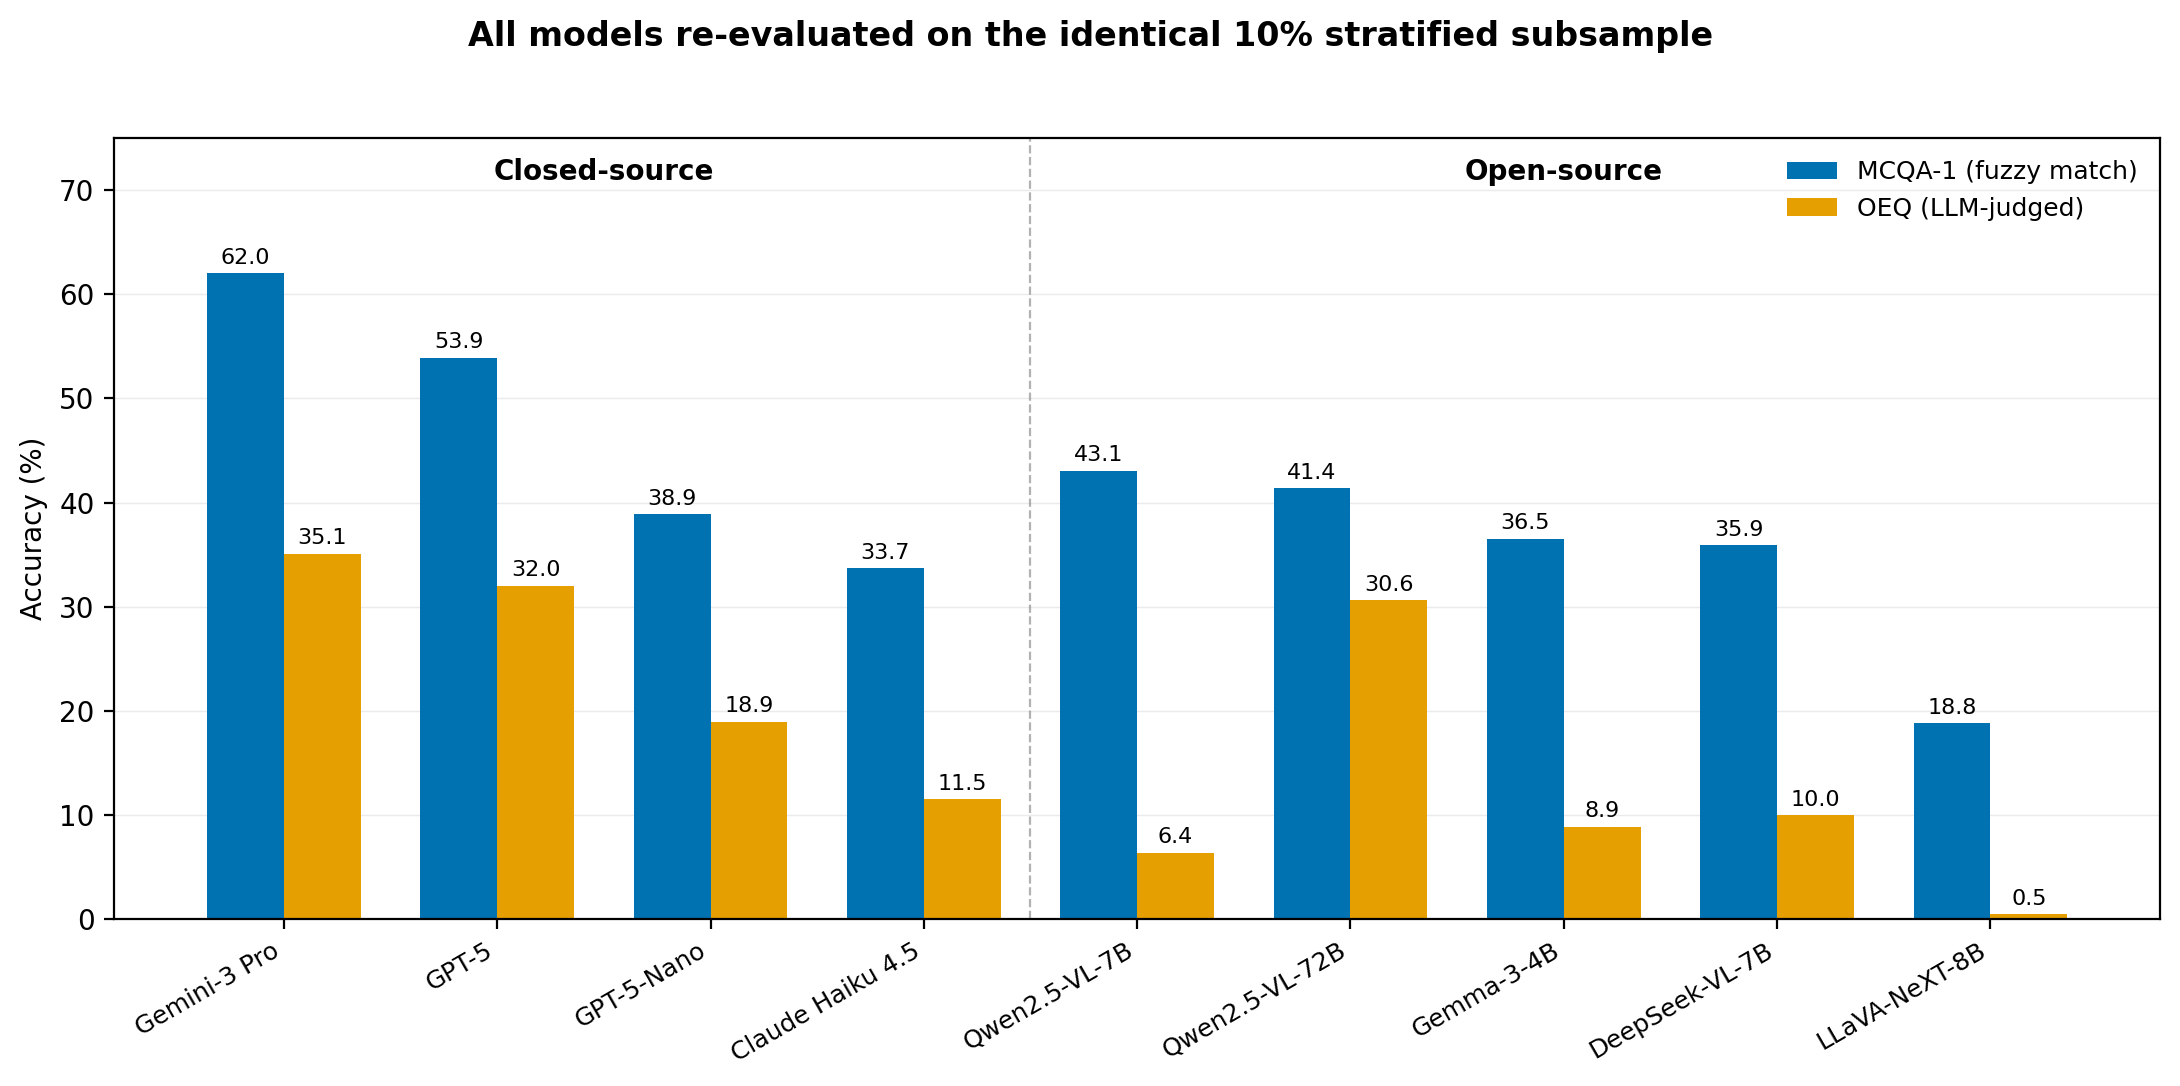
\includegraphics[width=\linewidth]{subsample_all_models.png}
    \caption{Every model's overall accuracy (mean across disease, pest/damage, and weed task groups, matching the aggregation in Table~\ref{tab:main_results}) recomputed on the identical 10\% stratified subsample, for MCQA-1 (fuzzy match) and OEQ (LLM-judged). Models evaluated on the full dataset in the main text (Qwen2.5-VL-7B, Gemma-3-4B, DeepSeek-VL-7B, LLaVA-NeXT-8B) are filtered to the same subset used for the closed-source models; no new inference was performed.}
    \label{fig:subsample_all_models}
\end{figure}

Figure~\ref{fig:subsample_all_models}\ confirms both orderings hold under this uniform footprint. MCQA-1 exceeds OEQ for every one of the nine models with no exception, including the four models that were not previously subsampled. The closed-vs-open-source ordering also holds at the extremes that anchor our main claims: Gemini-3 Pro and GPT-5 (the two best closed-source models) outperform every open-source model in both formats, and Qwen2.5-VL-72B (the best open-source model) remains behind them. The ordering is less clean-cut in the middle of the distribution: Qwen2.5-VL-7B and Qwen2.5-VL-72B (43.1\% and 41.4\% MCQA) both outperform GPT-5-Nano and Claude Haiku 4.5 (38.9\% and 33.7\%) under this uniform subsample, so ``closed-source outperforms open-source'' should be read as a property of the strongest models on each side rather than a strict per-model ordering, consistent with our existing discussion of Qwen2.5-VL-72B approaching closed-source performance (Section~\ref{sec:results}). Comparing these subsample-based numbers to the full-dataset values already reported for the four newly-filtered models (Table~\ref{tab:main_results}) also provides four additional data points for the subsampling validation itself: MCQA-1 accuracy shifts by at most 0.76pp between the full dataset and the 10\% subset (Qwen2.5-VL-7B: 46.64\% $\to$ 46.00\%; Gemma-3-4B: 40.61\% $\to$ 40.75\%; DeepSeek-VL-7B: 39.50\% $\to$ 38.77\%; LLaVA-NeXT-8B: 18.60\% $\to$ 19.36\%), consistent with the 0.9pp gap already reported for Qwen2.5-VL-72B in Section~\ref{sec:results}.

\end{document}
